\documentclass[12pt]{book}
\usepackage[width=4.375in, height=7.0in, top=1.0in, papersize={5.5in,8.5in}]{geometry}
\usepackage[pdftex]{graphicx}
\usepackage{amsmath}
\usepackage{epigraph}
\usepackage{amssymb}
\usepackage{setspace}
\usepackage{tipa}
\usepackage{tgbonum}
\usepackage{dirtree}
\usepackage[hidelinks]{hyperref}
\usepackage{textcomp}
\usepackage{amsthm}
% axiom through Axiomthm
\newtheorem{axiomthm}{Axiom}[chapter]
% Definition through "definition"
\newtheorem{definition}{Definition}[chapter]
% theorem through theorem
\newtheorem{theorem}{Theorem}[chapter]
\usepackage{array}
\usepackage{xy}
\usepackage{fancyhdr}
\usepackage{listings}
\usepackage{xcolor}  % for syntax highlighting colors
\usepackage{tcolorbox} % A more modern package for frame and background



% Define the color palette based on the Vim "desert" scheme
\definecolor{desertbackground}{HTML}{333333}
\definecolor{desertcomment}{HTML}{98FB98}
\definecolor{desertkeyword}{HTML}{87CEEB}
\definecolor{desertstring}{HTML}{F0E68C}
\definecolor{deserttext}{HTML}{FFFFFF}
% Set global style options for all listings
\lstset{
    basicstyle=\ttfamily\small,
    breaklines=true,
    breakautoindent=true,
    captionpos=t,
    frame=single,
}

% Define a specific style for FORTRAN
\lstdefinestyle{FORTRAN}{
    language=[95]Fortran,        % Use Fortran 95 syntax
    backgroundcolor=\color{desertbackground},
    basicstyle=\color{deserttext}\ttfamily\small,
    keywordstyle=\color{desertkeyword}\bfseries,
    commentstyle=\color{desertcomment}\itshape,
    stringstyle=\color{desertstring},
    numberstyle=\tiny\color{gray},
    numbers=left,
    captionpos=t,
    frame=single,
    showstringspaces=false,
    breaklines=true,
}

\usepackage{titlesec}  % for custom section levels

% Define new level
\titleclass{\subsubsubsection}{straight}[\subsubsection]
\newcounter{subsubsubsection}[subsubsection]
\renewcommand\thesubsubsubsection{\thesubsubsection.\arabic{subsubsubsection}}

% Format heading in text
\titleformat{\subsubsubsection}
  {\normalfont\normalsize\bfseries} % font style
  {\thesubsubsubsection}{1em}{}     % numbering
\titlespacing*{\subsubsubsection}{0pt}{1ex plus .1ex minus .2ex}{0.5ex} % spacing

% Define ToC level & indentation
\makeatletter
\def\toclevel@subsubsubsection{4} % level below subsubsection
\def\l@subsubsubsection{\@dottedtocline{4}{8em}{4em}} % indentation in ToC
\makeatother



% Increase numbering and toc depth
\setcounter{secnumdepth}{4}  % numbers subsubsubsection
\setcounter{tocdepth}{4}     % shows subsubsubsection in ToC
\pagestyle{fancy}
\renewcommand{\chaptermark}[1]{\markboth{#1}{}}
\renewcommand{\sectionmark}[1]{\markright{\thesection\ #1}}
\fancyhf{}
\fancyhead[LE,RO]{\bfseries\thepage}
\fancyhead[LO]{\bfseries\rightmark}
\fancyhead[RE]{\bfseries\leftmark}
\renewcommand{\headrulewidth}{0.5pt}
\renewcommand{\footrulewidth}{0pt}
\addtolength{\headheight}{0.5pt}
\setlength{\footskip}{0in}
\renewcommand{\footruleskip}{0pt}
\fancypagestyle{plain}{%
\fancyhead{}



\renewcommand{\headrulewidth}{0pt}
}
%
%\parindent 0in
\parskip 0.05in
%
\begin{document}
\frontmatter
%
\chapter*{\Huge \center Axiom}
\thispagestyle{empty}
%{\hspace{0.25in} \includegraphics{./ru_sun.jpg} }
\section*{\huge \center AJ Cason}
\setcounter{secnumdepth}{8}
\setcounter{tocdepth}{8}


%
%
\tableofcontents
%
\mainmatter
\input{Into}
% part 1
\part{The Foundation}
\chapter{Introduction}
As mentioned in the preface, this section is made to axiomatically develop the foundations needed. 

To illustrate, in order to develop physical theories, mathematics must be developed, a philosophy of science must be made, metaphysics, epistemology, and formal logic. Thus, a complete theory of all of these things and more should be created. One that has fundamental, expressible axioms. 

Also, most of these theories rely on one another, so a logical chronology must be defined. At the moment of writing this it is defined to be logic $\to$ metaphysics $\to$ Epistemology$\to$ philosophy of science $\to$
philosophy of physics $\to$ mathematics $\to$ physics $\to$  theology $\to$ ethics $\to$ social philosophy $\to$ personal philosophy.

One additional thing to add, you may notice the separation of metaphysics and the philosophy of physics. These are both meant to signify a difference where metaphysics represents extremely fundamental questions like does existence exist. Things that must be answered before epistemology can be fully introduced. The next section, philosophy of physics, are slightly less fundamental, like the ontology of entropy. Questions that require a theory of epistemology to be answered. 

\chapter{Logic}
% Insert quote here
% Extra line
\singlespacing
\section{Introduction}
Logic is an important tool for the creation of all formal systems. It is the foundation of mathematics, which is for the most part the foundation of everything else. It is also simply important to anything else by clarify concepts, giving them formal definitions, and insures consistency. Allowing for a bedrock behind all analytical thinking. 

Though, before I can get into it too much, I should define what the study of logic is. It is the branch of philosophy that critically examines the fundamental nature, scope, and principles of logic itself.

It has a couple fo subfields as well. 
\begin{itemize}
    \item Philosophy of Logic
    \begin{itemize}
        \item The study of logic at a high level, analyzing its nature and scope.
    \end{itemize}
    \item Formal Logic
    \begin{itemize}
        \item A creation and usage of symbolic logic symbols to create systems; mainly mathematics.
    \end{itemize}
    \item Metalogic
    \begin{itemize}
        \item The technical, mathematical study of the properties of formal logical systems. The philosophy of logic often uses the results of metalogic (like Gödel's incompleteness theorems) to address its conceptual questions, such as the limits of a formal axiomatic system
    \end{itemize}
\end{itemize}
\section{Defining an Axiom}
This entire text is named Axiom, for it is the foundation. To define systems axiomatically and then build them out into their true complexity is not only one of my favorite things to do, but as an extension of that it is what this book is trying to do.(Obviously, I wouldn't do something like this if I didn't enjoy it.)

So let's define it. As I mention extensively in my last book, Lógos, we must define things extremely rigorously. By testing against edge cases and keep it with consistent.

A good way to start is with the dictionary definition. "a statement accepted as true as the basis for argument or inference." For instance, our understanding of scientific realism is the understanding of the fact that our observations of reality are accurate.

A more defined definition can then be defined to say that an axiom is a statement that either cannot be proved or cannot be proved currently that is used within a greater statement that can be proved upon its edifice. These axioms, while don't require 'proof' generally desire some type of reasoning even if it is not objective or purely analytical in nature. For instance, the above arguments for the objective nature of reality aren't true objective proof, they still exist as semi-arguments. While we cannot prove the objectivity of reality with true and objective reasoning, some reasoning can be applied to get some kind of 'proof' of the statement so that further studies can be applied based upon that said axiom.

An astute observer can find that these mean the same thing, my is more of an explanation so, the dictionary definition does work:
\begin{definition}
    Axiom: a statement accepted as true as the basis for argument or inference.
\end{definition}
\section{Formal Logic}
Let us start with formal logic, a system of symbols to be able to represent logic. Then build from there.
\subsection{Classical logic}
The most basic form of logic is classical logic, the examination of simple singular objects.
\subsubsection{Propositional logic}
The most basic form of classical logic, but instead of telling you now, I will develop it.
\subsubsection{Truth Tables}
Negation is the first an simplest form. The symbol is $\neg$, so $\neg A$ is the negation of A.

so the table can be constructed
$$A \quad \neg A$$
$$T \quad F$$
$$F \quad T$$
Where T, represents true, and F represents false.

A further complication is the conjunction operator $\land $ or "and." It combines to functions into a greater set.(a union of function)
\begin{align*}
    A \quad B \quad A\land B \\
    T \quad T \quad \quad T \quad \\
    T \quad F \quad \quad F \quad \\
    F \quad T \quad \quad F \quad \\
    F \quad F \quad \quad F \quad
\end{align*}
$A \land B$ is only true when both "A" and "B" are true.

$\lor$ is the inverse, only one of the functions must be true. It is called a disjunction. 
\begin{align*}
    A \quad B \quad A\lor B \\
    T \quad T \quad \quad T \quad \\
    T \quad F \quad \quad T \quad \\
    F \quad T \quad \quad T \quad \\
    F \quad F \quad \quad F \quad
\end{align*}

$A \implies B$ means "if A, then B" meaning that A needs to happen for B or that A causes B.
\begin{align*}
    A \quad B \quad A\implies B \\
    T \quad T \quad \quad \quad T \quad \quad  \\
    T \quad F \quad \quad \quad T\quad \quad \\
    F \quad T \quad \quad \quad  F \quad \quad \\
    F \quad F \quad \quad \quad  T \quad \quad
\end{align*}

\chapter{Metaphysics}

\chapter{*Epistemology}

\chapter{Philosophy of Science}

\chapter{Philosophy of Physics}

\chapter{Physics}

\chapter{Foundations of Mathematics}

\chapter{Theology}

\chapter{Ethics}

\chapter{Social Philosophy}

\chapter{Personal Philosophy}


% part 2
\part{Notes}
\chapter{Introduction}

\chapter{Textbooks}
\section{Introduction}
Here I will write my notes from books I have read or am reading.
\section{Theoretical Physics by Georg Joos}
\par The vector analysis portion is intresting due to the fact that it takes something as simple as vector analysis and brings rigorous ideas to it like that $\oint ds=0 $ for close surfaces. 
\par I also never really thought about using vector analysis instead of tensors. 
\par The rest of curl, gauss, and such is very simple. Though, now it is getting into tensors though vectors.
$$dv_x=ds\nabla v_x$$
$$dv_y=ds\nabla v_y$$
$$dv_z=ds\nabla v_z$$
\par So therefore $dv=ds \nabla v$
\par To calculate v, three vectors or nine scaler must be known.
\par Another interesting addition is the fact that in physics, symmetric tensors can be represented as a surface to the second degree.
\par One thing I have noticed is I need a more intuitive grasp into the relationships between curl, div, laplance, and grad. They use it a lot to simplify the calculations. 
$$\nabla^2 f = \nabla \cdot (\nabla f)$$
The Laplace operator is equal to the divergence of the gradient.
$$\nabla \times (\nabla f) = 0$$
For smooth scaler fields. The curl of the gradient is zero.
$$\nabla \cdot (\nabla \times \mathbf{F}) = 0$$
The same is true for the divergence of the curl.
$\nabla^2 \mathbf{F} = \nabla(\nabla \cdot \mathbf{F}) - \nabla \times (\nabla \times \mathbf{F})$
For vector fields, the Laplace operator has different relations.
\\
\par Next, onto calculus of variations. I will derive Euler-Lagrange differential equation.
\par Let: $\tilde{y}$ be a neighboring function to $y$. Where $\in$ be a small quantity and $\eta(x)$ be a arbitrary function of x. so if $\tilde{y}=y+\epsilon \eta$ then $\tilde{y'}=y'+ \epsilon \eta'$. Here we stipulate that the two functions $\tilde{y}$ and $y$ converge at the beginning and end. Thus, $\eta$ must vanish at the ends. So if we substitute an integral $I$,, we find that it becomes a function of $\epsilon$. Then we require that $I(\epsilon)$ must have an extreme value of $\epsilon=0$. Here it is in mathematical terms:
$$I(\epsilon)=\int^{x_1}_{x_0}F(x,y+\epsilon \eta, y'+\epsilon\eta')dx=extremum \ for \ \epsilon=0$$
\par This gives us a simple way of determining the extreme value for a given integral. The condition is:
$$(\frac{dI}{D\epsilon})_{\epsilon=0}=0$$
\par We can then expand the integrad function $F$ in Taylor's series, according to the powers of $\epsilon$.
\par The differentiate with respect to $\epsilon$.
\par This expression then vanishes for $\epsilon=0$. Thus then simply remains the condition for the extremum.
\par Integrate this to get the Euler-Lagrange differential equation:
$$\frac{d}{dx}\frac{\partial F(x, y, y')}{\partial y'}-\frac{\partial F(x, y, y')}{\partial y}=0$$
\\
\par For writing constraining forces, we find it to be 
$$Z=\lambda \ grad \ G$$
\par Where $G(x,y,z)$ is the equation of the surface
\\

\section{On Sympathetic Reduction in Classical Mechanics}
\section{Magnetic Fields and Magnetic Diagnostics for Tokamak Plasmas by Alan Wooton}
\section{Advanced MHD with Applications to Laboratory and Astrophysical Plasmas by Cambridge }
\par For wide variety of MHD instabilities operating in tokamaks, represented by normal modes of the form(assuming that  cylindrical approximation and the toroidal representation may be ignored):
$$f(\psi,\vartheta, \varphi, t)=\sum\nolimits_m \tilde{f}(\psi) e^{i(m\vartheta + \eta \varphi - \omega t)} $$
\par Is only unstable for perpendicular wave vectors.
\par The reason is the enormous field line bending energy of the Alfven waves

\section{Hamiltonian description of the ideal Fuid by P.J.Morrison}
 \section{Classical Dynamics a Modern Perspective}
 \subsection{Chapter 6}
 A lot more importation stuff I forgot to write down, well I will start in chapter 6:
 If multiple canonical transformations, directly transforming would be canonical. $w \to w' \to w''$ then $w \to w''$. This is the group Composition Law.
 
 Next is the Associativity of Composition Law: 
 if $w’= \phi(w)$, $w” = \Phi(w’)$, and $w’'' = \xi(w")$
 so no matter what order of transformation they will be the same, whether ($T_3(T_2T_2)$ or $(T_3T_2)T_1$ or anything of the such.
 
 Identity: The identity transformation w’ = w obviously obeys the conditions for being canonical.

Inverses: If $\omega \to \omega’$ is canonical, then so is the transformation 
id $\omega’ \to \omega$. 

"Thus all the properties needed to define a group are trivially obeyed. (In 
Chapter 12 we discuss group structure in a little more detail). "

The canonical group is characterized by the dimension, 2k, 
of the phase space. 

The subgroups of such a phasespace is very large, though three can be easily defined.

Another subgroup is the contact transformations.(when a poission bracket can be formed)

Note: changing coordinate systems can satisfy phasespace rules, but isn't generally considered to be a transformation

"Intuitively speaking, a finite canonical transformation that can be 
connected continuously to the identity should be built up as a succession of 
infinitesimal transformations."

To express the relation between Poission Brackets and canonical transformations through differential equations:
$$\frac{d \omega}{d \theta}= \{\omega^\mu, \phi(\omega)\}_\omega= \epsilon^{\mu v}\frac{\partial \phi(\omega)}{\partial \omega^v}$$

Let us first clarify the meaning of this equation. We look upon the $w^\mu$ as 
functions of $\theta$; $\phi$ is a function with a fixed functional form, and $w^\mu$ are the unknowns in the differential equation. Thus on the right-hand side of this equation, the arguments of $\phi$ are just the quantities we are trying to solve for. From the theory of differential equations, we know that there is a unique solution for $w^\mu$ if we are given the values of $w^\mu$ at $\theta = 0$. Calling these boundary values of $w^\mu$ as $w^\mu_0$, the solution of the equation can be written as: 
$$\omega^\mu= \varphi^\mu(\omega_0; \theta), \space \space \space \varphi^\mu(\omega_0; 0) = \omega^\mu_0$$

\subsection{Chapter 7}

\chapter{Coding}
\section{*Linux Terminal}

\section{*Github}

\section{*FORTRAN}

\section{*Python}


% Part 3
\part{Notes}
\chapter{Introduction}

\input{../text/part_3/prev_work}
\chapter{The Structure of Motion: A Philosophical Journey Through Hamiltonian Mechanics}
“The Hamiltonian formalism of mechanics, especially in its canonical form, has been an inexhaustible source of inspiration for modern theoretical physics.” | Albert Einstein
\section{Introduction}
\par This chapter is planned to be an extreme examination of Hamiltonian mechanics, especially from a philosophical, logic, and abstract way. Eventually, it will go from the basic logic and axioms underlying it, to the metaphysics and epistemology that are derived, and finally to advanced and modern usages. The primary purpose of this exercise is for me to find the gaps in my knowledge and gain a more intuitive and deep understanding of these concepts.(It was also written in 10th grade before the rest of the book so may not have the same standards.)
\par The reasoning for this is due to the extremely complex and abstract nature of such mechanics. To see the world through 'flows' instead of forces.
\subsection{Physical Reality and Frameworks}
\par Now, there are many theories, models, descriptions, framework, and so much more. Though, what really differentiates them? What makes one thing one and the other the other. While I won't truly go into extreme linguistic detail for every single one, I will go into moderate detail within the art to get the general idea down.
\par Let's focus on frameworks, because that is what a Hamiltonian is(others define it as schemes which is another great word and arguably more accurate, but I will refer to it as a framework because it has a more intuitive grasp). It is an entirely different framework than Newtonian. It comes from an entirely different perspective, looking into geometric identities rather than the causal relation of forces and such interactions. Also, other theories and identities are derived through it, independent of the actual reality of it. For instance, the flow of electromagnetic interactions, relativistic, or even gravitational are all derived from this concept of the flow of energies through sympathetic geometry. 
\par Even beyond that, Hamiltonian mechanics can represent any function that changes; statistics, viruses, and many others. This is due, to that Hamiltonian's is a pure mathematic relational concept rather than based upon physical axioms. For instance, Newtonians is based upon the axiom of inertia. Though, I will add one interesting involvement is the idea of privileging Hamiltonian over Lagrangian and stating that Lagrangian is a subset of Hamiltonian rather than its own framework.
\par Then this begins to ask our questions of scientific realism vs anti-realism(I found out the more neutral language is instrumentalism). Basically, what makes such theories more fundamentalist, predictive modeling or metaphysical truth. Further, this now engages the complexities of mathematical axiomatic reduction or physical.
\par Let's start with realism vs instrumentalism. I have already made my stance clear, having metaphysical truth in important but not in the way that non-metaphysical schemes should be thrown away. Though, this then brings about the question of what frameworks have greater metaphysical truth, but I will later look into this in later sections. 
\par This now leads to the question of mathematical abstraction vs physical realism. Though, one thing I will add is that the physical axioms of Newton's laws are based upon falsified ideas like absolute space and time(but you can get around such semantics by employing Whewell's axioms of Mechanics[1st: “Every change is produced by a cause.”
2nd says that: “Causes are measured by their effects.” Finally, the third remain unchanged from Newton's formulation.] Now back to the main event, I feel that the structuralism of Hamiltonian is better due to the fact that when you break down physics to the quantum the classical forces, inertia, and such break down and you can see that the structure is what remains. That while forces still interact as abstract 'causes of change" through bosons, their classical and 'physical' realism fails to encapsulate their extreme complexity.

\subsection{Philosophical Context*}
\par The Kantian influence on Sir Hamilton is clear....
\subsection{Notion of Time, States, and Trajectories}
\par Let's start with time. I have already explained my thoughts on time, but here I will deepen my explanation. Time, is the factor on which states evolve. It is then evolution of entropy. This axiom is very simple and intuitive. While objective empirical proving the nature of time is extremely challenging due to its abstract nature. For a more in-depth analysis of the nature of time visit Chapter 1, section 3\&7.
\par One thing I will discuss is time reversibility. Now, Hamiltonian mechanics works best for time reversal symmetries(it can still work in some use cases but rarely.). In fact, time reversal symmetry is a corner stone of much of modern physics, especially quantum mechanics, but this interferes with our intuitive grasp of reality, the second law of thermal dynamics, and even dark energy; in essence the emergent properties of reality seem to interfere with our 'fundamental mathematical' derivations. So I will examen these questions; both for their own state and because it continues our question of the fundamental nature of reality. I will also attempt to discuss imaginary time with regards to quantum mechanics.
\par Actually, upon further thought the nature of time will be further developed through after the derivation of analytical mechanics.
\par Next will the on trajectories; now like many other ideas presented within this book, that may seem simple but the derivation of the ideas will be thorough and show its true complexity. Within Hamiltonian mechanics, the trajectories hold special geometric identities due to the nature of motion, but what can we derive from this simple observations

\subsection{Introduction to Phase Space}
\par Another question that arises from a Hamiltonian view of metaphysics is Phase Space. The fact that, according to our theories, phase space almost seems real, but yet it is so very different than what we observer. Or, we think so.
\par Obviously, there is the idea of the conflict between the teleology that comes as a consequence and our view of causality. I will address this in a second.
\par A simpler idea is that, from a perspective view, change becomes fundamental and any identity becomes simply emergent. This isn't truly new, simply more emergent in phase space, so I will move on.
\par One new thing, is that Phase Space allows for entropy irreversibility. Traditional theories find time reversibility to be a corner stone, this going against it.
\par This is due to the fact that entropy increases
$$S=-k_B\Sigma_i p_i logp_i$$
Where the volume of the phase space stays the same
$$Vol(\phi_t(\Omega_M))=Vol(\Omega_M)$$

\par Lastly, the 6D phase space seems very different to ours. Having generalized position and momentum coordinates is odd. An instrumentalist view makes this simple, but a scientific realism makes this difficult. Sadly, I don't have the knowledge to come up with.
\subsection{Teleology vs Causality}
\par My privileging of causal relations has already become clear, but now I will justify my thoughts through a Hamiltonian view point. While many claim that the nature of Hamiltonian mechanics necessitates a teleology, and my stated view on structuralism seems to contradict my views on causality, but I will address these claims categorically.
\par First, the nature of Hamiltonian mechanics necessitates a teleological view of the natural world. This statement will seemingly logical, lacks the tautological strength required of such an extreme statement. For one, Hamilton himself had a clear belief in causality(while this obviously isn't enough, I will explain why he and I see it that way.) First, the concepts of causal forces(forces are by definition causation principles) can be derived through the inverse gradient of potential energy. Second, the connection of the 'principle of least' action and teleology is flimsy at best. This is because their main argument is based upon intuition of mathematic alone not physical realism(I know this goes against stated structuralism but I will come back to that), the reason I state this against due to the fact that, mathematical intuition in the face of metaphysical truth. For instance, as stated earlier the teleological 'energy' is found as a derivation of causal force. Finally, returning to our arguments placed in the first chapter.
\subsection{Role of Variational Principles in Mechanics}
\section{Axiomatic Mechanics}
\subsection{Axiomatic Derivation of ... }
\subsubsection{Introduction}
\par For any mathematical physical axiomatic derivation, a mathematical derivation is first required. I won't go super in depth but I will still go over it for rigors sake. I may go back and do a deeper dive but for now I will simply put these things.
\subsubsection{Axiom of Real numbers}
Why needed: Physical quantities like position, velocity, time, energy, and action are represented by real numbers. The calculus used in mechanics relies on the properties of real numbers.
\\
Key axioms:
\begin{itemize}
    \item Commutative, associative, and distributive properties for addition and multiplication. 
    \item Existence of additive and multiplicative identities (0 and 1).
    \item Existence of additive and multiplicative inverses (for non-zero numbers).
    \item Completeness axiom: Every non-empty set of real numbers with an upper bound has a least upper bound (ensures continuity, critical for calculus).
\end{itemize}



Role: These axioms enable arithmetic operations, inequalities, and the construction of functions like the Lagrangian $ L(q, \dot{q}, t) $.

\subsubsection{Axiom of Euclidean Geometry}
Why needed: If the system involves spatial coordinates (e.g., particles moving in 3D space), Euclidean geometry provides the framework for defining positions and distances.
\\
Key axioms(informal):
\begin{itemize}
    \item Points, lines, and planes exist.
    \item A straight line can be drawn between any two points.
    \item Distance between points is defined (e.g., via the Pythagorean theorem).
\end{itemize}

Role: Defines generalized coordinates $ q $ (e.g., Cartesian or polar coordinates) and kinetic energy terms like $ \frac{1}{2} m \dot{x}^2 $.
Note: For abstract systems (e.g., in generalized coordinates), geometry may be less critical, but it’s foundational for physical intuition.

\subsubsection{Axiom of Set Theory (Basic)}
Why needed: Sets are used to define the domain of variables (e.g., time $ t \in \mathbb{R} $, coordinates $ q \in \mathbb{R}^n $) and functions.
\\
Key axioms(informal):
\begin{itemize}
    \item Existence of sets: Sets can be formed to represent collections of objects (e.g., possible paths of a system).
    \item Union, intersection, and Cartesian product: Allow combining and manipulating sets.
    \item Axiom of choice (implicitly): Ensures a choice of path exists in variational problems.

\end{itemize}

Role: Provides the language for defining functions, spaces, and the configuration space of a system.

\subsubsection{Axiom of Calculus (Differential and Integral Calculus)}
Why needed: The principle of stationary action involves integrals (action $ S = \int L \, dt $) and derivatives (in Euler-Lagrange equations).
\\
Key concepts (built on axioms of real numbers):
\begin{itemize}
    \item Limits: Define continuity and differentiability of functions like $ L(q, \dot{q}, t) $.
    \item Derivatives: Partial derivatives (e.g., $ \frac{\partial L}{\partial q} $) are used to describe rates of change.
    \item Integrals: The Riemann integral defines the action $ S $.
    \item Fundamental theorem of calculus: Links derivatives and integrals, essential for variational calculus.

\end{itemize}

Role: Enables the formulation of the action and the variation $ \delta S = 0 $.
\subsubsection{Axioms of Variational Calculus}
Why needed: The principle of stationary action requires finding the path that makes the action stationary, which is a problem in variational calculus.
\\
Key axioms(informal):
\begin{itemize}
    \item Functional: The action $ S $ is a functional (a function of functions, e.g., paths $ q(t) $).
    \item Variation: Small changes in the path $ \delta q(t) $ are used to compute $ \delta S $.
    \item Stationary condition: The path satisfies $ \delta S = 0 $, leading to the Euler-Lagrange equations.

\end{itemize}

Role: Provides the mathematical machinery to derive the equations of motion from the action.

\subsubsection{Axioms of Linear Algebra (Basic)}
Why needed: For systems with multiple coordinates or degrees of freedom, vectors and matrices describe generalized coordinates $ q_i $ and momenta $ p_i $.
\\
Key axioms:
\begin{itemize}
    \item Vector space axioms: Addition and scalar multiplication of vectors (e.g., coordinates in $ \mathbb{R}^n $).
    \item Linearity: Operations like partial derivatives in Hamilton’s equations are linear.


\end{itemize}
Role: Supports the formulation of the Hamiltonian $ H(q, p, t) $ and phase space (the space of $ (q, p) $).

\subsubsection{Axioms of Variational Calculus}
Why needed: The principle of stationary action requires finding the path that makes the action stationary, which is a problem in variational calculus.
\\
Key axioms(informal):
\begin{itemize}
    \item Functional: The action $ S $ is a functional (a function of functions, e.g., paths $ q(t) $).
    \item Variation: Small changes in the path $ \delta q(t) $ are used to compute $ \delta S $.
    \item Stationary condition: The path satisfies $ \delta S = 0 $, leading to the Euler-Lagrange equations.

\end{itemize}

Role: Provides the mathematical machinery to derive the equations of motion from the action.

\subsubsection{Physical Assumptions (Not Strictly Mathematical Axioms)}
While not mathematical axioms, certain physical assumptions are mathematically formalized:
\begin{itemize}
    \item Time is continuous and one-dimensional ($ t \in \mathbb{R} $).(Though Hamiltonains can work in other forms)
    \item Energy is well-defined: Kinetic energy $ T $ and potential energy $ V $ are functions of coordinates and velocities.
    \item Differentiability: The Lagrangian $ L $ is sufficiently smooth (at least twice differentiable) to allow partial derivatives
    \item 

\end{itemize}
Role: These ensure the mathematical framework applies to physical systems.
\subsection{Axiomatic Derivation of Hamiltonian Mechanics}
% Introducing Hamilton's contribution
Two hundred years ago, William Rowan Hamilton reformulated classical mechanics using the \textbf{principle of stationary action}, a single axiom that unifies the dynamics of physical systems. This principle states that the path taken by a system between two times makes the action \( S \) stationary.

% Defining the action and Lagrangian
The \textbf{action} is defined as:
\[
S = \int_{t_1}^{t_2} L(q, \dot{q}, t) \, dt,
\]
where \( L = T - V \) is the \textbf{Lagrangian}, with \( T \) as kinetic energy, \( V \) as potential energy, \( q \) as generalized coordinates, and \( \dot{q} \) as their time derivatives.

% Deriving the Euler-Lagrange equations
The system follows the path where \( \delta S = 0 \). Varying the action:
\[
\delta S = \int_{t_1}^{t_2} \left( \frac{\partial L}{\partial q} \delta q + \frac{\partial L}{\partial \dot{q}} \delta \dot{q} \right) dt = 0.
\]
Integrating by parts on the second term:
\[
\int_{t_1}^{t_2} \frac{\partial L}{\partial \dot{q}} \delta \dot{q} \, dt = \left. \frac{\partial L}{\partial \dot{q}} \delta q \right|_{t_1}^{t_2} - \int_{t_1}^{t_2} \frac{d}{dt} \left( \frac{\partial L}{\partial \dot{q}} \right) \delta q \, dt.
\]
Since \( \delta q = 0 \) at \( t_1, t_2 \), we get the \textbf{Euler-Lagrange equations}:
\[
\frac{d}{dt} \left( \frac{\partial L}{\partial \dot{q}} \right) - \frac{\partial L}{\partial q} = 0.
\]

% Introducing the Hamiltonian
Hamilton defined the \textbf{Hamiltonian} as:
\[
H(q, p, t) = \sum_i \dot{q}_i p_i - L(q, \dot{q}, t),
\]
where \( p_i = \frac{\partial L}{\partial \dot{q}_i} \) are generalized momenta. Typically, \( H = T + V \).

% Deriving Hamilton's equations
Using the Legendre transform, the dynamics are governed by \textbf{Hamilton's equations}:
\[
\dot{q}_i = \frac{\partial H}{\partial p_i}, \quad \dot{p}_i = -\frac{\partial H}{\partial q_i}.
\]

% Example application
\textbf{Example}: For a particle in gravity, \( L = \frac{1}{2} m \dot{h}^2 - mgh \). The momentum is \( p = \frac{\partial L}{\partial \dot{h}} = m \dot{h} \). The Hamiltonian is:
\[
H = \frac{p^2}{2m} + mgh.
\]
Hamilton's equations yield:
\[
\dot{h} = \frac{p}{m}, \quad \dot{p} = -mg,
\]
reproducing the equation of motion \( m \ddot{h} = -mg \).

% Significance
The principle of stationary action simplifies dynamics, applies to diverse systems, and underpins modern physics, including quantum mechanics and relativity. Hamilton's work remains a cornerstone of theoretical physics.
\subsection{*Hamiltonian Mechanics ad a Geometric Theory}
\subsection{*Poisson Brackets and the Algebra of Dynamics}
\subsection{*Canonical Transformations: Symmetry, Simplicity, an Structure}

\section{Philosophical Implications*}
\subsection{*Time in Essence}
\subsection{*Hamiltonian Constraints and the Problem with Time}

\section{Modern Hamiltonian}
\subsection{Modern Research}
\subsubsection{*Hamiltonian Formulation in Plasma Physics}
\subsubsection{*Hamiltonian and Metriplectic Mechanics}
\subsubsection{*Symplectic Integrators: Preserving the Structure of Nature}
\subsubsection{*HNNN(Hamiltonian Neural Networks)}
\subsection{Fun Mess Around}
\subsubsection{Non-Canonical Poisson Brackets}
\par A Poisson bracket is a bilinear, antisymmetric operation $[F, G]$ that defines the time evolution of a functional $F$ via $\dot{F} = [F, H]$, where $H$ is the Hamiltonian.  Non-canonical brackets arise when the phase space variables (e.g., density, velocity, magnetic field in MHD) do not follow the standard canonical structure $\{q_i, p_j\} = \delta_{ij}$. 
\\
Properties: The bracket must satisfy:
\\
\begin{itemize}


    \item Antisymmetry: $[F, G] = -[G, F]$
    \item Leibniz Rule: $[F, GH] = [F, G]H + G[F, H]$
    \item Jacobi Identity: $[F, [G, H]] + [G, [H, F]] + [H, [F, G]] = 0$
\end{itemize}
\par For this I will be defining my own Poisson bracket specifically for plasma thrusters.
\par For this I will obviously need to define the variables. Things like:
\begin{itemize}
    \item Mass density: $\rho(\mathbf{r}, t)$
    \item Velocity field: $\mathbf{v}(\mathbf{r}, t)$
    \item Magnetic field: $\mathbf{B}(\mathbf{r}, t)$
    \item Entropy or internal energy: $s(\mathbf{r}, t)$ or $\epsilon(\rho, s)$
\end{itemize}
\par Now define the Hamiltonian, for this I will use the pre-established ideal-MHD, but in all reality for plasma thrusters I should use a more expanded model.
$$H[\rho, \mathbf{v}, \mathbf{B}, s] = \int \left( \frac{1}{2} \rho v^2 + \rho \epsilon(\rho, s) + \frac{B^2}{2\mu_0} \right) d^3x$$
\par Next, I must define the phase spaces and constraints. Incompressibility or magnetic field divergence. 
\par Next I propose a bracket system, with many of them being 
$$[F, G] = \int \sum_{i,j} \frac{\delta F}{\delta \xi_i} J_{ij} \frac{\delta G}{\delta \xi_j} d^3x$$
\par Such that Ideal MHD is:
$$[F, G] = -\int \Bigg\{
\rho \left[ \frac{\delta F}{\delta \rho}, \frac{\delta G}{\delta \mathbf{v}} \right]
+ \left[ \frac{\delta F}{\delta \mathbf{v}}, \frac{\delta G}{\delta \mathbf{v}} \right] \cdot \left( \frac{\mathbf{B}}{\rho} \times \nabla \times \frac{\delta G}{\delta \mathbf{B}} \right)
+ \frac{1}{\rho} \left( \nabla \times \frac{\delta F}{\delta \mathbf{B}} \right) \cdot \left( \frac{\delta G}{\delta \mathbf{v}} \times \mathbf{B} \right)
+ s \left[ \frac{\delta F}{\delta s}, \frac{\delta G}{\delta \mathbf{v}} \right]
\Bigg\} d^3x$$
\par Another approach is using lie-groups. The Lie-Poisson approach is a method to construct non-canonical Poisson brackets by reducing a canonical Hamiltonian system on a large phase space (e.g., particle coordinates) to a smaller phase space of collective variables (e.g., fluid fields in MHD). It is rooted in the symmetry properties of the system’s configuration space, described by a Lie group.
\par ...
\par The other way is through Casmir invariants. Casimir invariants are functionals $C$ that commute with all functionals $F$ under the Poisson bracket: $[C, F] = 0$. They are conserved quantities that arise from the degeneracy of the non-canonical bracket and provide constraints on the system’s dynamics.
\par Degeneracy: Non-canonical Poisson brackets are degenerate, meaning their Poisson tensor $J_{ij}$ has a non-trivial kernel. Casimirs live in this kernel, satisfying:
$$J_{ij} \frac{\delta C}{\delta \xi_j} = 0$$

\par Physical Role: Casimirs represent invariants tied to the system’s topology or symmetries, such as helicity in MHD, which constrain the evolution of plasma in thrusters.
\par Identification: Casimirs are found by solving the functional equation $[C, F] = 0$ for all $F$, often using the Lie algebra’s cohomology.

\chapter{Omega-X}
\section{Pre-planing(part 1)}
\subsection{Ideas \& Overarching Plan}
\par Start with replicating 1D thermal fluid model, then start with more complex models, then experiment with other ways to do it, then dive deeper into the mathematics and hopefully come up with something(maybe metriplectic integrator), then create a code base, compare these systems to other traditional models, and create tokomak simulation(maybe, not sure if possible yet) that is it so far. Hopefully these ideas will evolve. 

Basically, the whole idea is to create a Flash-X like project with Metriplectic formulism underlying the the dynamics rather than lagrangian or Newtonian. Obviously much simpler though.

\subsection{Metriplectic 4-bracket algorithm for constructing thermodynamically consistent
 dynamical systems}
\subsubsection{Math}
1: Identify dynamical variables
2: Propose energy and entropy functionals
3: Find Poisson bracket ${F, G}$ for which entropy $S$ is a Casimir invariant, ${F, S} = 0 \forall F$
4: Construct metriplectic 4-bracket (F, K; G, N) via Kulkarni-Nomizu product by a new method that separates local thermodynamics from phenomenological quantities, giving the EoMs as Poisson bracket + 4-bracket

To find the $\Sigma$ and $M$ a new method is derived. 
$$\partial_t \xi^\alpha= \{\xi^\alpha , H\} + \nabla \cdot J^\alpha$$
$\alpha = 1, 2... N-1$
$$\partial_t \xi^N= \{\xi^N , H\} + \nabla \cdot J^N+Z_\alpha \cdot \tilde{L}^{\alpha \beta} \cdot Z_\beta$$
where $\xi_N = \sigma$, the entropy density. Above splits Hamiltonian and conservative.
Which leads to:
$$M(dF, dG)=F_{\xi N}G_{\xi N}$$
$$\Sigma(dF, dG)=\nabla F_{\xi \alpha }\frac{L^{\alpha \beta}}{H_{\xi N}}\nabla (G_{\xi \beta})$$
\subsection{A thermodynamically consistent discretizations of 1D thermal-fluid
models using their metriplectic 4-bracket structure}
\subsubsection{Math}
Edit: so I don't keep forgetting, $\rho$ is mass density, $m$ is momentum density, and $\sigma$ is entropy density. Then for the thermodynamic quantities: $\eta$ is specific entropy, $u$ is velocity, and $T$ is temperature 
 Let $V_h = v_h \subset H^1(\Omega)$ be the degree-p continuous
 Galerkin finite element space defined over a uniform grid, $\tau_h $, on Ω: i.e.
 $$V_h = {v_h  \in H^1(\Omega) : v_h|K \in P_p(K), \forall K \in T_h}$$
  The discretizations is accomplished
 using the method of lines by positing that all dynamical fields have spatial dependence modeled
 in this Galerkin subspace. However, rather than discretizing the equations of motion themselves,
 we discretize the weak forms implied by the metriplectic formulation.
\\
 Let $(\rho_h. m_h. \sigma_h) \in V_h \times V_h \times V_h$
 So that the discretized Hamiltonian and entropy can be given as:
 $$H^h[\rho_h. m_h. \sigma_h]= \int_\Omega [\frac{1m^2_h}{2 \rho_h}+\rho_h U (\rho_h, \frac{\sigma_h}{\rho_h}]dx$$
 $$S^h[\sigma_h]=\int_\Omega \sigma_h dx$$
 Then the Metriplectic 4 Bracket can be expressed through:
 $$(F^h, K^h, G^h, N^h)_h = -\frac{1}{\text{Re}} \int_{\Omega} \frac{1}{T_h} \left[ \left( K^h \partial_x F^h_{m_h} - F^h \partial_x K^h_{m_h} \right) \right], $$
 $$\left( N^h \partial_x G^h_{m_h} - G^h \partial_x N^h_{m_h} \right)  \\
 +, $$
$$ \frac{1}{\text{Pr} \gamma - 1} \frac{1}{T_h} \left( K^h \partial_x F^h - F^h \partial_x K^h \right) \left[ \left( N^h \partial_x G^h - G^h \partial_x N^h \right) \right] \, dx $$
\\
Then the poission bracket is thus:
\begin{align*}
\{F^h, H^h\}_h(u_h)= - (m_h \partial_x u_h, \phi_m)_{L^2} + (m_h u_h, \partial_x , \phi_m)_{L^2} - \\ (\rho_h \partial_x \eta_h, \phi_m)_{L^2}  + (\rho_h u_h, \partial_x , \phi_\rho)_{L^2} - (\sigma_h\partial_x T_h, \phi_m)_{L^2} + (\sigma_h u_h, \partial_x, \phi_\sigma)_{L^2}
\end{align*}
Now, one thing I will say is that this is not technically a Poisson bracket, because it is fails to satisfy the Jacobi identity. This is because it is impossible(or at least nobody has figured out a way to discretize fluid poission brackets.

To then find equations of motion, adding them together $F^h=\{F^h, H^h\}_h+(F^h, H^h; S^h, H^h)_h$ where $F^h$ is the observable. 

In the case of momentum we must let $\phi_\rho = \phi_\sigma = 0$ so that only $\phi_\rho$ the momentum test function in the finite element(FE) test space $V_h$.

\begin{align*}
    (\phi_m, \partial_tm_h) + (m_h\partial_xu_h, \phi_m)_{L^2} - (m_h u_h, \partial_x, \phi_m)_{L^2}
    + (\rho_h \partial_x \eta_h, \phi_m)_{L^2} + (\sigma_h\partial_xT_h \phi_m)_{L^2} +
    \frac{1}{Re}(\partial_xu_h, \partial_x, \phi_m)_{L^2} = 0 
\end{align*}
\\
Next, I will have $\phi_m=\phi_\sigma=0$ to get continuity equations:
\\
\begin{align*}
    (\phi_\rho, \partial_g \rho_h)_{L^2}-(\rho_hu_h, \partial_x \phi_\rho)_{L^2}
\end{align*}

Finally the entropy equation is derived in a similar fashion:

\begin{align*}
    (\phi_\sigma, \partial_g \sigma_h)_{L^2}-(\sigma_h u_h, \partial_x \phi_\sigma)_{L^2}+\frac{1}{Re}[(\frac{(\partial_x u_h)^2}{T_h}, \phi_\sigma)_{L^2}-\frac{1}{Pr}\frac{\gamma}{\gamma-1}[(\frac{\partial_x T_h}{T_h}, \partial_x\phi_\sigma)_{L^2}-(\frac{(\partial_x T_h)^2}{T_h^2}, \phi_\sigma)_{L^2} ]]
\end{align*}

To prove energy conservation
$$(\frac{u^{n+1}_h-u^n_h}{\Delta t}, \delta h_h)=\frac{H(u^{n+1}_h)-H(U^n_h)}{\Delta t} = 0$$
Positive entropy production can be found through:
$$\frac{s^{n+1}_h-s^n_h}{\Delta t} = \frac{1}{Re}[(\frac{(\partial_x u^n_h)^2}{T^n_h},1)_{L^2}+\frac{1}{Pr}\frac{\gamma}{\gamma-1}\frac{(\partial_x T^n_h)^2}{T^n_h},1)_{L^2}]\geq 0$$


Let's figure out all we need to find for each equation, starting with momentum. 
Start with $M_{ii}=\phi_m$, this should be equal to dx, but I will confirm. Also need the time derivative of the momentum variational, $u_h$ variational, $\rho_h$ variational, $T_h$, $\eta_h$, and $\frac{1}{Re}$, reynolds number, decide later

$$M_{ii}=dx$$
$$u_h=(\rho_h, m_h, \sigma_h)$$
$\rho_h$, $T_h$, and $\eta_h$ are the respective fields, initialized simply and evolved through the equation.
Obviously $\rho_h, m_h,$ and $\sigma_h$ evolve through their metriplectic equations of "motion."
$T_h$, $\eta_h$, are evolved through these equations:
$$(\eta_h + \frac{m^2_h}{2\rho^2_h}-U(\rho_h, \frac{\sigma_h}{\rho_h})-\rho_h \partial_1 U(\\rho_h, \frac{\sigma_h}{\rho_h})+\frac{\rho_h}{\sigma_h}\partial_2U(\rho_h, \frac{\sigma_h}{\rho_h}, \phi_\eta)_{L^2}=0$$
$$(u_h-\frac{m_h}{\rho_h},\phi_u)=0$$
$$(T_h-\partial_2U(\rho_h, \frac{\sigma_h}{\rho_h})\phi_T)_{L^2}=0$$
\\
Nothing new is added in continuity
\\
Entropy adds: $Pr$ and $\gamma$
\subsubsection{Coding}
The first thing is to use a Galerkin Method for projecting PDEs into a finite-dimensional function space. (can base off of Firedrake, FEniCS, Galerkin, or another) $M_{ii}$ in mesh.f90

The second thing to do is to initialize the parameters and states(use mesh to calculate field) in states.f90
($Pr$, $Re$, $\gamma$ for constants; initialize ($\rho_h, \sigma_h, m_h, \eta_h, T_h, u_h$)


Then functionals: calculates pointwise functional derivatives of the Total Hamiltonian and Entropy. in functionals.f90
(Update $\rho_h, \sigma_h, m_h, u_h$)

EOS.f90 is used to update the thermodynamic points($\eta_h, T_h$)

Time step the program, by using Gauss-Legendre implicit Runge-Kutta methods in time\_integration.f90

Run the Program(using the driver and makefile)

Input the outputs in io.f90

Some notes: $(f,g)_{L^2}=\int_\Omega f(x) \cdot g(x)$

An example would be, for a point in the momentum equation $(\phi_m, \partial_t m_h)_{L^2}$, or the mass matrix times the derivative of momentum functional as a function of time. Thus it makes it so $\phi_m=M_{ii}=dx$ thus, $(\phi_m, \partial_t m_h)_{L^2}=dx\cdot\frac{m_h}{\partial t}$

\subsubsection{Future Work}
The paper presents several ways to improve, or at least look into improving through future work.

Mainly, they mention that many different structure preserving methods exist and may be more suitable.

I also need to figure out how to make this codebase work for more examples



\subsection{Metriplectic Framework for
 Dissipative Magneto-Hydrodynamics}
\subsubsection{My Introduction}
In my time trying to figure out how to numerically solve metriplectic equations, someone beat me to dissipative magneto-hydrodynamics. Oh well, I can build off of.

Beyond that, the abstract introduces the paper better than I could,
" The metriplectic framework, which permits to formulate an algebraic structure for dissipative
 systems, is applied to visco-resistive Magneto-Hydrodynamics (MHD), adapting what had already
 been done for non-ideal Hydrodynamics (HD). The result is obtained by extending the HD sym
metric bracket and free energy to include magnetic field dynamics and resistive dissipation. The correct equations of motion are obtained once one of the Casimirs of the Poisson bracket for ideal MHD is identified with the total thermodynamical entropy of the plasma. The metriplectic frame work of MHD is shown to be invariant under the Galileo Group. The metriplectic structure also permits to obtain the asymptotic equilibria toward which the dynamics of the system evolves. This scheme is finally adapted to the two-dimensional incompressible resistive MHD, that is of major use in many applications."
\subsubsection{Notes on introduction}
They have an interesting word choice, "with its noble descendants of path integral representations," or Algebrization of dynamical systems appears to be the final destination of that virtuous route.

MSTDOF means "microscopic, statistically treated, degrees of freedom"

In this introduction they derive the metriplectic existence quite simply.
Starting with the poission bracket 
$$\dot{f}=\{f,g\}$$
In this case
$$0= \{S,H\}$$
Thus it is the Casimir functionals of the Poisson bracket
$$\{C,f\}=0 \forall f$$
From here we can define the Hamiltonian free energy. 
$$F=H+\lambda C $$
Where $\lambda$ is an arbitrary constant left. In MSTDOF, it is the minus of the tempeture.

To then expand the system, $\langle\langle f,g \rangle \rangle$ via $F$. So that $\langle\langle f, g\rangle \rangle=\{f,h\} + (f,g)$ and $(f,g)$ is symmetric, bilinear and semi-definite.

Evolution is then given by
$$\dot{f}=\langle\langle f, F\rangle \rangle$$
(the symmetric bracket $(f,g)$ will be defined so to cancel out the presence of the coefficient
 $\lambda$, removing it from the equations of motion).

 $(f,g)$ is defined so that $H$ is conserved.
 $$(H, f) = 0 \forall f$$
 Thus metriplectic evolution reads:
 $$\dot{f}=\{f,H\}+\lambda(f,C)$$
 The Casimir to mimic entropy undergoes an evolution described by:
 $$\dot{C}=\lambda(C,C)$$
 \\
 Now, I like this introduction. Clearly showing the basic understanding on Metriplectic dynamics.
 \subsection{METRIPLECTIC FORMULATION OF VISCO-RESISTIVE MHD}
 The system observed is fully ionized plasma. Where dissipation takes place due to the finite viscosity and resistivity of the fluid. Also, heat conductivity is finite. Here is the SO(3)-covariant form.(expressing physical equations in a way that is invariant under rotations in three-dimensional space)
 \begin{align*}
\partial_t \rho + \partial_i (\rho u^i) &= 0 \\
\partial_t B^i + \varepsilon^{ijk} \partial_j E_k &= 0, \quad \partial_i B^i = 0 \\
\partial_t (\rho u^i) + \partial_j (\rho u^i u^j + p \delta^{ij}) &= \varepsilon^{ijk} J_j B_k + \partial_j (\eta \, \partial_j u^i) \\
\partial_t s + \partial_i (s u^i) &= \frac{\eta}{T} \partial_i u^j \partial_i u^j + \frac{\kappa}{T^2} \partial_i T \partial_i T + \frac{\mu}{T} J^i J^i
\end{align*}
There is quite a bit to this equation, but I will move on.

One thing I will add is a new notation. $\dot{H}\overset{\partial}{=}0$, it simply means that means that $\dot{H}$ and 0 only differ by a boundary term.

They then describe the poission bracket for ideal MHD(when dissipation does not happen, thus traditional poission bracket).

This equation has multiple Casimir observables. The paper mentions:
$$C[\rho, s]=\int_\mathbb{D}\rho\varphi(s)d^3x$$
Which within is both the total mass and entropy.
$$M[\rho]=\int_\mathbb{D}\rho d^3x$$
$$S[\rho,s]=\int_\mathbb{D}\rho s d^3x$$
Thus, mass and entropy are conserved. There are some other, but obviously for this purpose, use the entropy.

Taking the dissipative equations from the to combine $D=(\vec{D}^\rho, \vec{D}^v, \vec{D}^B, \vec{D}^s)$ something called an 8-uple. So we must want to define our metriplectic bracket as $\psi = (\psi, D)$ where $\psi$ is the dynamic variables.

Uhm.. I just realized this wasn't the paper I thought it was. Good read, but I don't think I will continue these notes.
\subsection{A least Action principle for visco-resistive Hall Magnetohydrodynamic with metriplectic reformulation}
\subsubsection{Abstract}
The abstract persented says,

"We present a new variational formulation for Viscous and resistive Hall Magnetohydrodynamic. We first find a variational principle for ideal HMHD by applying the physical assumptions leading to HMHD at the lagrangian level, and then we add the viscous and resistive terms by the means of constrained variations. We also provide a metriplectic reformulation of our formulation, based on two canonical Lie-Poisson brackets for the ideal part and metric 4-brackets for the dissipative part."

They then go into all of these, I will begin with the Metriplectic for notes alone.
\subsubsection{Metriplectic bracket, Hamiltonian and Entropy for Viscoresistive Hall MHD}
They use the Inclusive curvaturelike tensor found in Morrison's recent work. Where the dissipation is included using a 4-bracket that have the same symmetries as a curvature tensor.

They take the assumption that the viscous  tensor can be found to be 
$$\sigma=\Lambda \nabla u_i$$
Where $\Lambda$ is symmetrize and positive.
\subsection{Variational discretizations of viscous and resistive
 magnetohydrodynamics using structure-preserving finite
 elements}
 \subsubsection{Abstract}
 We propose a novel structure preserving discretization for viscous and resistive magnetohy
drodynamics. We follow the recent line of work on discrete least action principle for fluid and
 plasma equation, incorporating the recent advances to model dissipative phenomena through
 a generalized Lagrange-d’Alembert constrained variational principle. We prove that our semi
discrete scheme is equivalent to a metriplectic system and use this property to propose a Poisson
 spliting time integration. The resulting approximation preserves mass, energy and the diver
gence constraint of the magnetic field. We then show some numerical results obtained with our
 approach. We first test our scheme on simple academic test to compare the results with estab
lished methodologies, and then focus specifically on the simulation of plasma instabilities, with
 some tests on non Cartesian geometries to validate our discretization in the scope of tokamak
 instabilities.

 
 This paper
\section{part 2}
\subsection{Coding(1D fluid)}
\paragraph{Introduction}
My first step to creating my codebase is to create it for the simplest form. This is specifically made for the purpose of figuring things out, documenting it, and such things. So, I will be writing down each file.

\paragraph{mesh\_1d}
Obviously, this mesh program creates the mesh for the program. The size $N$, the nodes $x\_nodes$ and the mass matrix $M_{ii}$. The rest are self explanatory but I will go into what the mass matrix is. It represents the discrete inner product of basis functions.
$$M_{ii}=(\phi_i,\phi_j)_{L^2}=\int_\Omega \phi_i(x)\phi_j(x)dx$$
So, $M_{ii} $ becomes a metric tensor for program. It turns continuous inner products into discrete sums over coefficients.

It can be approximated through the "lumped mass matrix" where $M_{ii}=dx$
Though, I use the trapezoidal mass matrix:
$$M_{ii}(1) = 0.5d0 * dx $$
$$ M_{ii}(N) = 0.5d0 * dx$$
$$M_{ii}(2:N-1) = dx$$
For more information visit, \url{https://arxiv.org/pdf/2008.03883}
\begin{lstlisting}[style=FORTRAN, caption=mesh\_1d.f90]
module mesh_1d
  implicit none
  private
  public :: initialize_mesh, x_nodes, dx, N, Mii

  ! Parameters
  integer, parameter :: N = 100         ! Number of spatial grid points (nodes)
  real(8), parameter :: L = 1.0d0       ! Length of the domain

  ! Mesh data
  real(8), dimension(N) :: x_nodes      ! Coordinates of each mesh node
  real(8) :: dx                         ! Uniform cell spacing

  ! Mass matrix (diagonal approximation here, for full FEM use full M)
  real(8), dimension(N) :: Mii          ! Lumped mass matrix diagonal

contains

  subroutine initialize_mesh()
    integer :: i

    dx = L / (N - 1)

    ! Initialize node positions
    do i = 1, N
      x_nodes(i) = (i - 1) * dx
    end do

    ! Lumped mass matrix: each diagonal entry is dx
    Mii = dx

    ! Uncomment below to use trapezoidal mass matrix
    Mii(1) = 0.5d0 * dx
    Mii(N) = 0.5d0 * dx
    Mii(2:N-1) = dx

  end subroutine initialize_mesh


end module mesh_1d 
\end{lstlisting}

\paragraph{states\_1d}
States then initializes the constants and fields.
First the constants(parameters) used throughout the code. Re, Reynolds numbers. $\gamma$, compression of the fluid. $Pr$, Prandtl number, ratio of viscous to thermal diffusion.

Then, it initializes the discretion fields of entropy, momentum, mass, temperature, and specific entropy.

This should be modularized for the future to make this codebase iterative.

Now, what exactly to do. I think for this, have constants in a separate one. Then for the fields, I am not sure at this moment.
\begin{lstlisting}[style=FORTRAN, caption=states\_1d.f90]
module states_1d
  use mesh_1d
  implicit none
  private
  public :: m_h, rho_h, sigma_h, eta_h, T_h
  public :: initialize_states

  ! Field arrays
  real(8), allocatable :: m_h(:)       ! Momentum density
  real(8), allocatable :: rho_h(:)     ! Mass density
  real(8), allocatable :: sigma_h(:)   ! Entropy density
  real(8), allocatable :: eta_h(:)     ! Specific entropy (diagnostic)
  real(8), allocatable :: T_h(:)       ! Temperature (diagnostic)
  real(8), parameter, public :: gamma = 1.4
  real(8), parameter, public :: Pr = 0.71
  real(8), parameter, public :: Re = 1000.0

contains

  subroutine initialize_states()
    implicit none
    integer :: i

    ! Allocate fields
    allocate(m_h(N))
    allocate(rho_h(N))
    allocate(sigma_h(N))
    allocate(eta_h(N))
    allocate(T_h(N))

    ! Set initial conditions (example: Gaussian density bump)
    do i = 1, N
      rho_h(i) = 1.0d0 + 0.2d0 * exp(-100.0d0 * (x_nodes(i) - 0.5d0)**2)
      eta_h(i) = 1.0d0
      sigma_h(i) = rho_h(i) * eta_h(i)
      m_h(i) = 0.5d0
      T_h(i) = (0.4d0) * eta_h(i)  ! Ideal gas ! Uses EOS
    end do

  end subroutine initialize_states

end module states_1d
\end{lstlisting}
\paragraph{projection\_matrix\_1d}
Here the creation of two subroutines to simplify future calculations.
First, initialize\_projection\_matrix(), that simply creates matrix.
Next, apply\_weak\_derivative(f, d\_proj). This does:
$$proj=\sum_{i=1}^n(\sum_{j=1}^nD_{i,j})*f$$
Where $f$ is the observable.
For future work, I think all I need to do for this one is create multiple for different dimensions.
\begin{lstlisting}[style=FORTRAN, caption=projection\_matrix\_1d.f90]
module projection_matrix_1d
  use mesh_1d
  implicit none
  real(8), allocatable :: D(:,:)
  public :: initialize_projection_matrix, apply_weak_derivative

contains

  subroutine initialize_projection_matrix()
    integer :: i
    real(8) :: dphi_dx
    if (allocated(D)) then
      deallocate(D)
    end if

    allocate(D(N, N))
    D = 0.0d0

    dphi_dx = 1.0d0 / dx

    ! Loop over elements and assemble D
    do i = 2, N-1
      ! Local contributions from basis functions over each element
      D(i, i-1) = -dphi_dx / 2.0d0
      D(i, i  ) =  0.0d0
      D(i, i+1) =  dphi_dx / 2.0d0
    end do

    ! Optional: Neumann (zero derivative) at boundaries
    D(1,:) = 0.0d0
    D(N,:) = 0.0d0
  end subroutine initialize_projection_matrix

  ! Applies D to f to compute (phi_i, partial_x f)
  subroutine apply_weak_derivative(f, d_proj)
    implicit none
    real(8), intent(in)  :: f(N)
    real(8), intent(out) :: d_proj(N)
    integer :: i

    d_proj = 0.0d0
    do i = 1, N
      d_proj(i) = sum(D(i,:) * f(:))
    end do
  end subroutine apply_weak_derivative

end module projection_matrix_1d
\end{lstlisting}
\paragraph{mass\_1d}

\begin{lstlisting}[style=FORTRAN, caption=mass\_1d.f90]
module mass_1d
  use mesh_1d
  use projection_matrix_1d
  implicit none
contains

  subroutine compute_mass_flux(N, rho_h, u_h, rho_rhs)
    integer, intent(in) :: N
    real(8), intent(in) :: rho_h(N), u_h(N)
    real(8), intent(out) :: rho_rhs(N)
    real(8) :: flux(N)
    integer :: i

    ! Compute flux
    do i = 1, N
      flux(i) = rho_h(i) * u_h(i)
    end do

    ! Apply weak derivative
    call initialize_projection_matrix()
    call apply_weak_derivative(flux, rho_rhs)

    ! Divide by dx
    do i = 1, N
      rho_rhs(i) = -rho_rhs(i) / dx
    end do

    ! Boundary conditions
    rho_rhs(1) = 0.0d0
    rho_rhs(N) = 0.0d0

  end subroutine compute_mass_flux

end module mass_1d
\end{lstlisting}
\paragraph{momentum\_1d}
\begin{lstlisting}[style=FORTRAN, caption=momentum\_1d.f90]
module momentum_1d
  use states_1d, only: Re
  use mesh_1d
  use projection_matrix_1d
  implicit none
contains

  subroutine compute_momentum_rhs(N, rho_h, m_h, sigma_h, eta_h, T_h, rhs_m)
    integer, intent(in) :: N
    real(8), intent(in) :: rho_h(N), m_h(N), sigma_h(N), eta_h(N), T_h(N)
    real(8), intent(out) :: rhs_m(N)
    real(8) :: u_h(N), du_proj(N), mu(N), dmu_proj(N), deta_proj(N), dT_proj(N)
    integer :: i

    ! Compute velocity
    do i = 1, N
      if (rho_h(i) > 1.0d-12) then
        u_h(i) = m_h(i) / rho_h(i)
      else
        u_h(i) = 0.0d0
      end if
    end do

    ! Apply weak derivatives
    call initialize_projection_matrix()
    call apply_weak_derivative(u_h, du_proj)
    do i = 2, N-1
      mu(i) = m_h(i) * u_h(i)
    end do
    call apply_weak_derivative(mu, dmu_proj)
    call apply_weak_derivative(eta_h, deta_proj)
    call apply_weak_derivative(T_h, dT_proj)

    ! Compute RHS
    do i = 2, N-1
      rhs_m(i) = 0.0d0
      rhs_m(i) = rhs_m(i) - m_h(i) * du_proj(i) * dx
      rhs_m(i) = rhs_m(i) + dmu_proj(i) * dx
      rhs_m(i) = rhs_m(i) - rho_h(i) * deta_proj(i) * dx
      rhs_m(i) = rhs_m(i) - sigma_h(i) * dT_proj(i) * dx
      rhs_m(i) = rhs_m(i) - (1.0d0 / Re) * du_proj(i) * dx
    end do

    ! Boundary conditions
    rhs_m(1) = 0.0d0
    rhs_m(N) = 0.0d0

  end subroutine compute_momentum_rhs

end module momentum_1d
\end{lstlisting}
\paragraph{entropy\_1d}
\begin{lstlisting}[style=FORTRAN, caption=entropy\_1d.f90]
module entropy_1d
  use states_1d
  use mesh_1d
  use projection_matrix_1d
  implicit none
contains

  subroutine compute_entropy_rhs(N, sigma_h, u_h, T_h, rhs_sigma)
    implicit none
    ! Dummy arguments
    integer, intent(in) :: N
    real(8), intent(in) :: sigma_h(N), u_h(N), T_h(N)
    real(8), intent(out) :: rhs_sigma(N)

    ! Local variables
    real(8) :: flux(N), dx_u(N), dx_T(N)
    real(8) :: visc_prod(N), heat_prod(N), heat_grad(N), heat_term(N)
    integer :: i

    ! Compute flux
    do i = 1, N
      flux(i) = sigma_h(i) * u_h(i)
    end do

    ! Apply weak derivatives
    call initialize_projection_matrix()
    call apply_weak_derivative(flux, rhs_sigma)
    call apply_weak_derivative(u_h, dx_u)
    call apply_weak_derivative(T_h, dx_T)

    ! Viscous and thermal terms
    do i = 1, N
      visc_prod(i) = (dx_u(i)**2) / T_h(i)
      heat_grad(i) = dx_T(i) / T_h(i)
      heat_prod(i) = (dx_T(i)**2) / (T_h(i)**2)
      heat_term(i) = (gamma / (gamma - 1.0d0)) * (heat_prod(i) - heat_grad(i) / dx)
      rhs_sigma(i) = rhs_sigma(i) - (1.0d0 / Re) * visc_prod(i) * dx
      rhs_sigma(i) = rhs_sigma(i) - (1.0d0 / (Re * Pr)) * heat_term(i) * dx
    end do

    ! Divide by dx
    do i = 1, N
      rhs_sigma(i) = -rhs_sigma(i) / dx
    end do

    ! Boundary conditions
    rhs_sigma(1) = 0.0d0
    rhs_sigma(N) = 0.0d0

  end subroutine compute_entropy_rhs

end module entropy_1d
\end{lstlisting}
\paragraph{velocity\_1d}
\begin{lstlisting}[style=FORTRAN, caption=velocity\_1d.f90]
module velocity_1d
  use states_1d
  use projection_matrix_1d
  implicit none
contains

  subroutine compute_velocity(N, rho_h, m_h, u_h)
    implicit none

    ! Dummy arguments
    integer, intent(in) :: N
    real(8), intent(in) :: rho_h(N), m_h(N)
    real(8), intent(out) :: u_h(N)

    ! Local variables
    integer :: i
    real(8), parameter :: eps = 1.0d-12  ! Small number to avoid division by zero

    ! Compute velocity safely
    do i = 1, N
      if (rho_h(i) > eps) then
        u_h(i) = m_h(i) / rho_h(i)
      else
        u_h(i) = 0.0d0
      end if
    end do

  end subroutine compute_velocity

end module velocity_1d
\end{lstlisting}

\paragraph{EOS\_1d\_thermal}

\begin{lstlisting}[style=FORTRAN, caption=EOS\_1d\_thermal.f90]
module eos_1d
  use states_1d
  implicit none
  private
  public :: compute_temperature, compute_eta



contains

  !------------------------------------------------------------
  ! Compute temperature T from specific entropy eta
  ! T = (gamma - 1) * eta
  !------------------------------------------------------------
  function compute_temperature(eta_h) result(T_h)
    real(8), intent(in) :: eta_h
    real(8) :: T_h

    T_h = (gamma - 1.0d0) * eta_h
  end function compute_temperature

  !------------------------------------------------------------
  ! Compute specific entropy eta from temperature
  ! eta = T / (gamma - 1)
  !------------------------------------------------------------
  function compute_eta(T_h) result(eta_h)
    real(8), intent(in) :: T_h
    real(8) :: eta_h

    eta_h = T_h / (gamma - 1.0d0)
  end function compute_eta

end module eos_1d
\end{lstlisting}
\paragraph{time\_integrator\_1d}
\begin{lstlisting}[style=FORTRAN, caption=time\_integrator\_1d.f90]
module time_integrator_1d
  use mesh_1d
  use states_1d
  use velocity_1d
  use eos_1d
  use mass_1d
  use momentum_1d
  use entropy_1d
  implicit none
  private
  public :: advance_one_step

contains

  subroutine advance_one_step(dt, u_h, rhs_m, rho_rhs, rhs_sigma)
    real(8), intent(in) :: dt
    real(8), intent(INOUT) :: u_h(N), rhs_m(N), rho_rhs(N), rhs_sigma(N)
    integer :: i

    ! Step 1: Compute velocity
    call compute_velocity(N, rho_h, m_h, u_h)
    
    ! Step 2: calculate tempeture
    do i = 1, N-1
      T_h(i) = compute_temperature(eta_h(i)) 
    end do
    ! step three: calculate Eta
    do i = 1, N-1
      eta_h(i) =compute_eta(T_h(i))
    end do
    ! Step 4: Compute Galerkin RHS terms
    call compute_momentum_rhs(N, rho_h, m_h, sigma_h, eta_h, T_h, rhs_m)
    call compute_mass_flux(N, rho_h, u_h, rho_rhs)
    call compute_entropy_rhs(N, sigma_h, u_h, T_h, rhs_sigma)

    ! Step 5: Advance in time (Euler / RK1)
    do i = 1, N
      m_h(i)     = m_h(i)     + dt * rhs_m(i)
      rho_h(i)   = rho_h(i)   + dt * rho_rhs(i)
      sigma_h(i) = sigma_h(i) + dt * rhs_sigma(i)
    end do

  end subroutine advance_one_step

end module time_integrator_1d
\end{lstlisting}
\paragraph{io\_1d}
\begin{lstlisting}[style=FORTRAN, caption=io\_1d.f90]
module io_1d
  use mesh_1d
  use states_1d
  use velocity_1d
  use time_integrator_1d
  implicit none
  private
  public :: write_state_to_csv

contains

  subroutine write_state_to_csv(filename)
    implicit none
    character(len=*), intent(in) :: filename
    integer :: i
    logical :: wait
    real(8) :: u_h(N)
    integer :: ierr
    
    ! Ensure the output directory exists
    wait = .true.  ! Command should run synchronously
    call execute_command_line("mkdir -p output", wait, ierr)
    if (ierr /= 0) then
        print *, "Error: Could not create output directory!"
        stop
    end if

    ! Compute velocity u = m / rho
    call compute_velocity(N, rho_h, m_h, u_h)

    ! Open file for writing
    open(unit=10, file=filename, status="replace", action="write", form="formatted")

    ! Header
    write(10, '(A)') 'x,rho,m,sigma,u,T,eta'

    ! Data
    do i = 1, N
      write(10, '(F12.6,1x,F12.6,1x,F12.6,1x,F12.6,1x,F12.6,1x,F12.6,1x,F12.6)') &
        x_nodes(i), rho_h(i), m_h(i), sigma_h(i), u_h(i), T_h(i), eta_h(i)
    end do

    close(10)
  end subroutine write_state_to_csv

end module io_1d
\end{lstlisting}
\paragraph{1D\_Thermal\_driver}
\begin{lstlisting}[style=FORTRAN, caption=momentum\_1d.f90]
program omega_x_driver_1d
  use mesh_1d
  use states_1d
  use time_integrator_1d
  use io_1d
  implicit none
  real(8) :: dt, t, t_end
  integer :: step = 1
  real(8), dimension(N) :: u_h, rhs_m, rho_rhs, rhs_sigma
  character(len=100) :: fname
  
  dt = 1.0d-3
  t_end = 1.0d0
  t = 0.0d0
  
  call initialize_mesh()
  call initialize_states()
  u_h = 0.0d0
  rhs_m = 0.0d0
  rho_rhs = 0.0d0
  rhs_sigma = 0.0d0  ! Explicitly initialize rhs_sigma here

  do while (t < t_end)
    call advance_one_step(dt, u_h, rhs_m, rho_rhs, rhs_sigma)
    t = t + dt
    print *, 't = ', t

    if (mod(step, 100) == 0) then
        write(fname, '(A,I4.4,A)') "output/state_", step, ".csv"
        call write_state_to_csv(fname)
    end if

    step = step + 1
  end do
end program omega_x_driver_1d
\end{lstlisting}
\subsubsection{Plans}
I have now create it in its most basic form, here are my next steps.

Break states up into constants and fields(multi-dimensional fields)

Make operators folder for projection, weak derivative, boundary conditions

Add checks(mainly energy conservation)

Upgrade time integration,(figure out)

Make different spacial discretization

More boundary conditions

Add more physics

Though, the main thing I need to work on is module registry + driver pattern. 
\section{part 3}
\subsection{Notes}
\subsubsection{Notes on module FORTRAN}
I should have a main driver like:
\begin{lstlisting}[style=FORTRAN, caption=Omegax.f90]
program Omegax
	use Driver_module
	implicit none

	call Driver_init()
	call Driver_evolve()
	call Driver_finalize()

end program Omegaz
\end{lstlisting}

There should also be a a config file, saying which modules should be used, and a python script capable of parsing this registery file.
Config would also be where parameters would be stored.
\subsubsection{Diminsionaless programing}
In the config file I can have a section to input the diminsions.

Then have all variable allocatable based upon the diminsions

then have an allocation based upon such diminsions(either preprocessor or generic shape handling)

Instead of hardcoding loops, create cases for different diminsions.


Generaliz derivatives and fluxes.

Also, while physics sections should be generalized, initializing between 3D, would be beneficial.
\subsubsection{Generalize}
Due to Metriplectics dyanmics complex mathematics, a fully generalized system, like FLASH-X, is impossible. This is because it is a dynamical theory based upon Hamiltonian Mechanics, rather than forces in Newtonian.

I am thinking the way to fix this is to create a symbolic python code to be able to generate the function I need.

Also, since these would be in py
\subsection{Plan}

I think the steps I am going to take are:

1: Develop a python code that can generate the math I need, I would also like for it to be able to read a LaTeX code for it.

2: I need to look into how to create a Config file for my problem at hand

3: Fix integration for this new system

4: 
\subsection{New Structure}
Here is the basic idea of what it should look like and do:
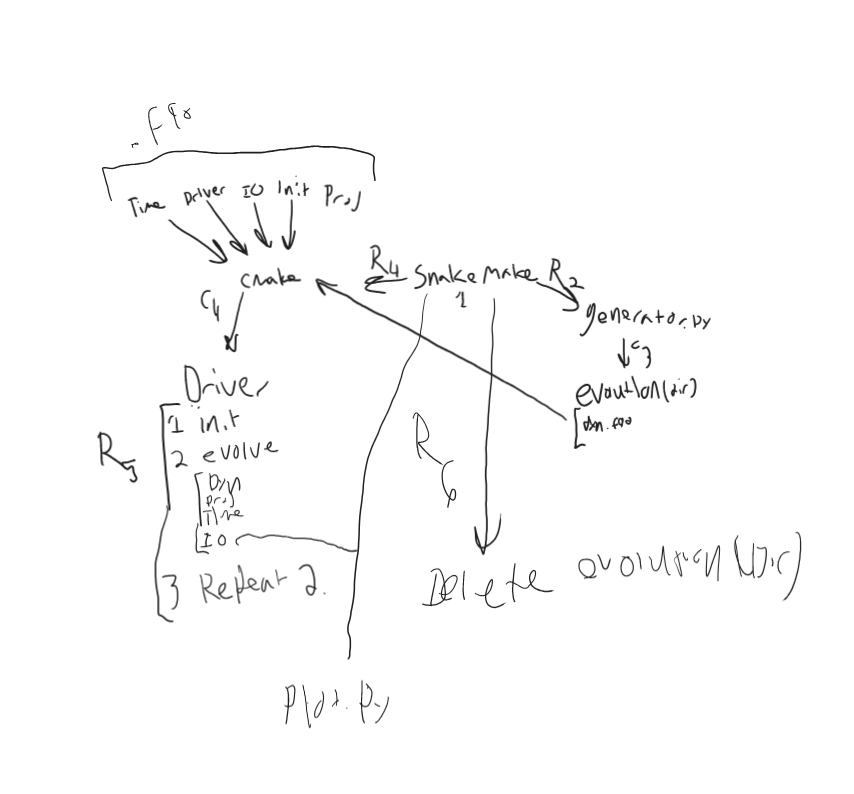
\includegraphics[width=1\textwidth]{../text/part_3/omega-x_overview.png}


\chapter{Axiom}
\section{*Structure}

\section{LaTeX}
\subsection{Division of Structure}
In this program I have used this structure to divide the book up:
\begin{verbatim}
    \part{}
    \chapter{}
    \section{}
    \subsection{}
    \subsubsection{}
    \subsubsubsection{} % custom made
    \paragraph
    \subparagraph
\end{verbatim}
I may have to learn new ways to divide in the future, but I will try to aviod that.
\subsection{Commands}
Here are some commands that I will have here for reference:
\begin{verbatim}
    \begin{verbatim} writes things exactly, used mostly 
    for writing LaTeX commands in this method
    \label{} → Set a reference point
    \ref{} → Refer to numbered items

    \pageref{} → Refer to page number

    \nameref{} (requires hyperref) → Refer to name/title 
    of chapter/section

    \autoref{} (requires hyperref) → Smart referencing 
    (automatically adds “Chapter”, “Section”)
    \begin{equation} ... \end{equation} → Numbered 
    equations

    \[ ... \] → Displayed, unnumbered equations

    $ ... $ → Inline math

    \frac{a}{b}, \sqrt{x}, \sum, \int → Standard 
    math symbols

    \begin{align} ... \end{align} (from amsmath) 
    → Multi-line aligned equations

    \begin{cases} ... \end{cases} → Piecewise functions

    \bra{}, \ket{}, \braket{} → 
    Use physics package for quantum notation

    \tensor{} → Use tensor package 
    for tensor indices

    \dv{}, \pdv{} → Derivatives (from physics)
    \begin{figure}[h!] ... \end{figure} → 
    Insert figures

    \includegraphics[width=0.8\textwidth]{file}
    → Image inclusion (graphicx)

    \caption{} / \label{} → Caption and reference

    \begin{table}[h!] ... \end{table} → Tables
\end{verbatim}

I also have begin\{lstlisting\} to write both FORTRAN and make. I will likely add python and Julia


% part 4
\part{Notes}
\chapter{Introduction}

\chapter{Plans}
\section{Now}
\subsection{Self-Education}
elf-education has always been a great value of mine. As mentioned earlier, I became obsessed with learning Einstein's field equation in 3-4th grade. Beyond that I have spent much of my time reading books, watching YouTube videos, and more about topics that interest me. Though, late in 8th grade, this desire to teach myself grew a great deal. Before I can go about my future goals for teaching myself I must first go over what I have already down.(This list is not full, mainly lectures finished and books from lectures, this does not include books not finished, non-lecture based video education, research papers read, projects where I learned things for the project alone, and other similar programs)
\\
Mathematics:
\begin{itemize}
    \item AP Calculus AB and BC - Khan Academy
    \item Multivariable Calculus 
    \item Khan Academy
    \item 18.03 Differential Equations - MIT OpenCourseWare
    \item Gilbert Strang on linear algebra - MIT OpenCourseWare
    \item Vector Calculus - Trevor Bazett
    \item Tensor Analysis - eigenchris
    \item Tensor Calculus - eigenchris
    \item Crash Course in Complex Analysis - Steve Burton 
    \item Introduction to Applied Numerical Analysis - Richard W. Hamming
    \item Symplectic geometry \& classical mechanics - Tobias Osborne 
    \item Lie groups, algebras, brackets - Mathemaniac (more conceptual than mathematical)
    \item Differential geometry - Robert Davie
    \item Calculus of variations - Faculty of Khan
    \item Working on
    \begin{itemize}
        \item Advanced Analytic Methods in Continuum Mathematics: Fundamentals for Science and Engineering - Hung Cheng 
        \item Discrete Differential Geometry - CMU
        \item Differential Geometry for students of Numerical Electrodynamics - Alain Bossavit
    \end{itemize}

\end{itemize}
Physics:
\begin{itemize}
    \item 8.02 Physics II - MIT OpenCourseWare
    \item 8.03 Physics III - MIT OpenCourseWare
    \item 8.033 Relativity - MIT OpenCourseWare
    \item General Relativity - Stanford Online
    \item Introduction to plasma physics - USYD senior plasma physics lectures
    \item Introduction to electromagnetism - Griffiths
    \item Computational physics - Mark Newman
    \item 8.224 Exploring Black Holes: General Relativity and astrophysics - MIT OpenCourseWare
    \item Classical Dynamics of Particles and Systems - Thornton Marion
    \item Introduction to cosmology - Stanford Online
    \item Introduction to fusion energy and plasma physics course - PPPL
    \item Seminar: Fusion and plasma physics - MIT OCW
    \item Statistical Mechanics - Stanford Online
    \item Hamiltonian description for magnetic field lines in fusion plasmas: A tutorial - AIP
    \item Fusion economics: power density, materials and maintenance - PPPL Frontiers Colloquia
    \item Flash-X code tutorial, a users perspective - University of Chicago(skimmed) 
    \item Flash-X user guide - Flash-x
    \item Flash4 User support(skimmed)
    \item Radiative Procuresses in Astrophysical Phenomena- George B. Rybicki, Alan P. Lightman
    \item Goldstien Classical Mechanics Lectures - Prof. Jacob Linder
    \item PiTP 2016 - Institute of Advanced study
    \item 2024 PPPL Graduate Summer School
    \item Hamiltonian description of the ideal Fuid - P.J.Morrison
    \item Quantum Mechanics with Applications - David B. Beard \& George B. Beard
    \item "What IS Structure, How Do You Create or Recognize It, and How Can You Use It? or Metriplectic Dynamics: Using the 4-Bracket for Constructing Thermodynamically Consistent Models." - workshop Geometric Mechanics Formulations for Continuum Mechanics
    \item "On an Inclusive Curvature-Like Framework for Describing Dissipation: Metriplectic 4-Bracket Dynamics." - workshop Infinite Dimensional Geometry and Fluids
    \item Haven’t finished
    \begin{itemize}
        \item Theoretical Physics - Georg Joos
        \item Advanced MHD with Applications to Laboratory and Astrophysical Plasmas - Cambridge
        \item Classical Mechanics: A Modern Perspective - Sudarshan and N. Mukunda
        \item The Interpretation of Structure From Motion - Ullman, S.
        \item Radiative Processes in Astrophysics - George B. Rybicki \& Alan P. Kightman
        \item Symplectic geometry \& classical mechanics - Tobias Osborne
    \end{itemize}

\end{itemize}
Coding:
\begin{itemize}
    \item Computational physics - Mark Newman
    \item Python Numerical Methods - Berkeley 
    \item Applied Numerical Methods - Crice Carnahan, H.A Luther, James O.Wilkes
\end{itemize}
Other:
\begin{itemize}
    \item Management in engineering - MITOpenCourseware
    \item Principles of microeconomics - MITOpenCourseware
    \item Dynamic leadership: using improvisation in business  - OpenCourseware
    \item Logic 1 - OpenCourseware
    \item Policy for science, technology, and innovation -  MITX
    \item Reducing The Danger Of Nuclear Weapons And Proliferation- MITOpenCourseware

\end{itemize}
\subsection{Research}
\begin{itemize}
    \item Egg drop simulation
    \item Numerical Methods for 3D compressed Plasma using Lattice Boltzmann(paper written)
    \item Simulated Annealing for plasma thrusters
    \item High Altitude EMP for primordial black holes(never finished) 
    \item Flash-x simulations:
    \begin{itemize}
        \item Basic Sedov
        \item Running simple MHD simulation of my own design
    \end{itemize}
    \item A Hamiltonian Framework on ICF Implosions Rocket Equation Based on Rayleigh-Taylor Instabilities
    \item Contributed to PlasmaPY
    \item Relativistic Rocket Equation(Newtonian)
    \item Relativistic rocket equation(Hamiltonian)
    \item Finite difference MHD Model in Fortran
    \item Computes velocity based upon Navier Stokes equation adapted to magnetic and electric fields
    \item Outputs graphical color field of velocity 
    \item Asteroid game
    \begin{itemize}
        \item Classical
        \item Time
        \item Survival
        \item Newtonian(player and asteroids have gravity)
        \item Dark Matter(Invisiable gravity fields)
        \item Relativistic(time dilation, spacial contraction, black holes, etc)
        \item Proximal Policy Optimization “AI” played game
    \end{itemize}
    \item Hamiltonian based plasma thruster Fortran Numerical Code
    \item N body simulation 
    \item Fluid based N-body simulation
    \item Death Star
    \begin{itemize}
        \item Basic gravitational ‘planet’
        \item MHD Plasma beam hitting
        \item Basic evaporation and kinetic energy transfer
    \end{itemize}
    \item OpenMHD usage
    \item Usage Gkyl
    \item Omega-X project
    \begin{itemize}
        \item Inspired by FLASH-X, attempting to build a multi-physics plasma physics codebase using Metriplectic forumism rather than Lagrandian and Newtonian
        \item I have successfully implemented the 1D thermofluid metriplectic discretization onto a discontinuous Galerkin subspace using an $L^2$ projection. Integrated using implicit midpoint rule.
        \item Working on module registry \& driver pattern
    \end{itemize}
\end{itemize}
\subsection{Other activities}
I also had some other activities that I have done in high school, I won't go too much in them. 
\begin{itemize}
    \item SVA
    \item Boy Scouts
    \item Church activities
    \item JROTC
    \item FCA
    \item OA
    \item Etc
\end{itemize}
The OA, Order of the Arrow, I will continue into college.
\section{Pre-University}
\subsection{Independent Learning}
One thing I need to do is nail calculus completely. I am going to be taking the AP calc BC test without taking the course. 

Beyond that, I am completing differential geometry. Once done I will finish Symplectic geometry. Then lie (brackets, algebra, group, and theory)

I also want to get into functional analysis.

I should also learn C++ beyond what I have done in the past.
\section{Undergrad}
\subsection{Classes}
\subsubsection{Requirments}
\subsubsubsection{General}
I have tested out of many of the general education requirements, so here is the remaining bit:
\begin{itemize}
    \item Written communication(pick 1)
    \begin{itemize}
        \item Honors ethical theory
        \item Haslam knowledge
    \end{itemize}
    \item Oral communication
    \begin{itemize}
        \item A survey in Contemporary Physics
    \end{itemize}
    \item Arts and humanities(pick 2)
    \begin{itemize}
        \item Haslam Knowledge
        \item honors intro to philosophy
        \item Professional responsibility
    \end{itemize}
    \item Civilization(pick 2)
    \begin{itemize}
        \item Honors development of Western civilization
        \item Honors history of world civilizations
        \item University Honors
        \item World Religions
    \end{itemize}
\end{itemize}
\subsubsubsection{Academic Physics Major}
\begin{itemize}
    \item Prerequisites
    \begin{itemize}
        \item Intro Computer Science
        \item Differential Equations 1
        \item Matrix Algebra
    \end{itemize}
    \item Core
    \begin{itemize}
        \item Fundamentals of modern physics
        \item Mechanics 1
        \item Thermal Physics
        \item Electronics Lab
        \item Intro to quantum mechanics
        \item Modern optics
        \item Electricity and Magnetism
        \item Survey in modern physics
        \item Modern Lab
        
    \end{itemize}
    \item Academic
    \begin{itemize}
        \item Mechanics 2
        \item Intro to quantum 2
        \item Electricity and magnetism 2
        
    \end{itemize}
    \item Recommended
    \begin{itemize}
        \item Mathematical Methods for scientist
        \item Partial Differential Equations
        \item Complex Variables
    \end{itemize}
    \item Thesis in physics
\end{itemize}
\subsubsubsection{Applied Maths Major}
\begin{itemize}
    \item Computer Science
    \item Core 
    \begin{itemize}
        \item Diff equations
        \item Matrix Algebra
        \item Intro to abstract mathematics
        \item Math proficiency
    \end{itemize}
    \item Breath
    \begin{itemize}
        \item Honors abstract algebra 1
        \item Honors Analysis 1
        \item Numerical Analysis
        \item Stochastic processes
    \end{itemize}
    \item Applied breath(physics courses)
    \item Depth
    \begin{itemize}
        \item Numerical Algebra
    \end{itemize}
\end{itemize}
\subsubsubsection{Computer Science Minor}
\begin{itemize}
    \item Intro comp sci
    \item data structures
    \item Logic design
    \item Numerical Algorithms
    \item Numerical Analysis
    \item Numerical Algebra
    \item Parallel Programming
\end{itemize}
\subsubsubsection{Electives}
\begin{itemize}
    \item PHYS 441 - Introduction to Computational Physics
    \item PHYS 494 - Special Topics in Physics 
    \item 2nd PHYS 493 - Research and Independent Study 
    \item PHYS 531 - Mechanics(Maybe, graduate)
    \item PHYS 541 - Electromagnetic Theory(Maybe)
    \item PHYS 571 - Mathematical Methods in Physics I(maybe)
    \item PHYS 573 Numerical methods in physics(maybe)
    \item PHYS 615 Astrophysics(maybe)
    \item PHYS 643 Computational Physics(maybe)
    \item MATH 462 - Differential Geometry
  	\item MATH 467 - Honors: Topology
    \item MATH 536 - Partial Differential Equations II
    \item MATH 567 - Riemannian Geometry I
    \item MATH 568 - Riemannian Geometry 2
    \item MATH 572 - Numerical Analysis II
    \item MATH 577 - Optimization
    \item MATH 579 - Seminar in Numerical Mathematics
\end{itemize}
\subsubsubsection{Total}
\begin{itemize}
    \item Honors ethical theory(x)

    \item honors intro to philosophy(x)
    \item Professional responsibility(x)
    \item Honors development of Western civilization(x)
    \item Honors history of world civilizations(x)
    \item Intro Computer Science(x)
    \item Differential Equations 1(x)
    \item Matrix Algebra(x)
    \item Fundamentals of modern physics(x)
    \item Mechanics 1(x)
    \item Thermal Physics(x)
    \item Electronics Lab(x)
    \item Intro to quantum mechanics(x)
    \item Modern optics(x)
    \item Electricity and Magnetism(x)
    \item Survey in modern physics(x)
    \item Modern Lab(x)
    \item Mechanics 2(x)
    \item Intro to quantum 2 x
    \item Electricity and magnetism 2 x
    \item Mathematical Methods for scientist(x)
    \item Partial Differential Equations x
    \item Complex Variables x
    \item Thesis in physics (x)
    \item Intro to abstract mathematics x
    \item Honors abstract algebra 1(x)
    \item Honors Analysis 1 (x)
    \item Numerical Analysis x
    \item Stochastic processes (x)
    \item Numerical Algebra(x)
    \item data structures(x)
    \item Logic design(x)
    \item Parallel Computing (x)
    \item 35(-1, -4, maybe) main(13-15 electives)
    \item MATH 462 - Differential Geometry(1)(x)
    \item MATH 467 - Honors: Topology(2)(x)
    \item PHYS 441 - Introduction to Computational Physics(15)
    \item PHYS 493 - Research and Independent Study(3)(x)
    \item PHYS 531 - Classical Mechanics(4)(x)
    \item PHYS 541 - Electromagnetic Theory(5)(x)
    \item PHYS 571 - Mathematical Methods in Physics I(6)(x)
    \item PHYS 573 - Numerical Methods in Physics(7)(x)
    \item MATH 515 - Analytical Applied Mathematics I(8)(x)
    \item MATH 567 - Riemannian Geometry I(9) x
    \item MATH 568 - Riemannian Geometry II(10) x
    \item MATH 569 - Seminar in Topology and Geometry(11)
    \item MATH 574 - Finite Element Methods(12)
    \item MATH 578 - Introduction to Scientific Computing(13) (x)
    \item MATH 585 - Optimal Control Theory(14)
    \item PHYS 599 - Seminars(x)
    \item PHYS 593 - Independent Study(x)
\end{itemize}
\subsubsection{Schedule}
\colorbox{yellow}{physics}
\colorbox{orange}{general}
\colorbox{green}{math}
\colorbox{red}{comp sci}
\subsubsection{First Year}
\begin{enumerate}
    \item  \colorbox{orange}{Honors ethical theory}
    \item  \colorbox{orange}{Honors intro to philosophy}
    \item  \colorbox{orange}{Professional Responsibility}
    \item  \colorbox{orange}{HR: Western Civilization}
    \item  \colorbox{orange}{HR: World civilization}
    \item  \colorbox{red}{Intro computer science}
    \item  \colorbox{green}{Diff equations 1}
    \item  \colorbox{green}{Matrix Algebra}
    \item  \colorbox{yellow}{Fundamentals in modern physics}
    \item  \colorbox{yellow}{mechanics 1}
    \item  \colorbox{green}{Intro to abstract mathematics}
    \item \colorbox{yellow}{PHYS 503 - Physics Colloquium}

\end{enumerate}
\subsubsection{Second Year}
\begin{enumerate}
    \item \colorbox{yellow}{Thermal Physics}
    \item \colorbox{yellow}{Electronics Lab}
    \item \colorbox{yellow}{Intro to quantum mechanics}
    \item \colorbox{yellow}{Modern optics}
    \item \colorbox{yellow}{Electricity and Magnetism}
    \item \colorbox{yellow}{Survey in modern physics}
    \item \colorbox{yellow}{Modern Lab}
    \item \colorbox{yellow}{Mechanics 2}
    \item \colorbox{yellow}{Intro to quantum 2}
    \item \colorbox{yellow}{Electricity and magnetism 2}
    \item \colorbox{green}{Partial Differential Equations}
    \item \colorbox{green}{Numerical Analysis}
    
\end{enumerate}
\subsubsection{Third year}
\begin{enumerate}
    \item \colorbox{green}{Honors abstract algebra 1}
    \item \colorbox{green}{Honors Analysis 1}
    \item \colorbox{green}{Stochastic Processes}
    \item \colorbox{green}{Numerical Algebra}
    \item \colorbox{yellow}{Mathematical Methods in physics}
    \item \colorbox{yellow}{Research \& independent study}
    \item \colorbox{green}{Differential Geometry}
    \item \colorbox{green}{Honors: Topology}
    \item \colorbox{yellow}{Classical Mechanics, grad}
    \item \colorbox{yellow}{PHYS 541 - Electromagnetic Theory, grad}
    \item \colorbox{green}{MATH 515 - Analytical Applied Mathematics I}
    \item \colorbox{yellow}{Independent study and research}
\end{enumerate}
\subsubsection{Fourth year}
\begin{enumerate}
    \item \colorbox{yellow}{Thesis in physics}
    \item \colorbox{green}{MATH 567 - Riemannian Geometry I}
    \item \colorbox{green}{MATH 568 - Riemannian Geometry II}
    \item \colorbox{yellow}{Numerical methods in physics}
    \item \colorbox{red}{data structures}
    \item \colorbox{red}{Logic design}
    \item \colorbox{red}{Parallel Computing}
    \item \colorbox{yellow}{PHYS 599 - Seminars}
    \item \colorbox{yellow}{PHYS 513 - Problems in Theoretical Physics I}
    \item \colorbox{green}{MATH 578 - Introduction to Scientific Computing}
    \item \colorbox{green}{MATH 534 - Calculus of Variations}
    \item \colorbox{green}{MATH 537 - Mathematical Principles of Continuum Mechanics I}
    
\end{enumerate}
\subsubsection{Others}
\begin{enumerate}
    \item PHYS 514 - Problems in Theoretical Physics II
    \item MATH 585 - Optimal Control Theory
    \item MATH 574 - Finite Element Methods
    \item PHYS 615 - Astrophysics and Cosmology(grad required)
    \item PHYS 643 - Computational Physics(grad required)
    \item MATH 515 - Analytical Applied Mathematics I
    \item MATH 571 - Numerical Analysis I
    \item MATH 572 - Numerical Analysis II
    
\end{enumerate}
\subsubsection{Possible summer}
\begin{enumerate}
    \item Graduate Reading in Mathematics
    \item Research and independent study
    \item graduate reading in physics
    \item Special Problems
\end{enumerate}
\section{*Grad}

\section{*Early career}

\section{*Late Career}


\chapter{Personal-Analysis}
"The unexamined life is not worth living" | Socrates
\section{Introduction}
I will use this journaling of sorts to examine myself and my own personality.
\section{Disgrace and Pride}
(if anyone else reads this, don't pay too much mind. I use words differently than their actual meaning. I don't word things very well. I was simply trying to capture my own indescribable and esoteric and possibly failable thoughts in this moment on this topic, my actual feelings are very different than what can be interpreted through the word choice.)(Additional update: upon later analysis, I have found that these ideas of pride and disgrace are for the most part the idea of seeing my earlier mentioned "personal values" in a light very similar to traditional morality. This doesn't fully explain it and I will continue to work on refining these ideas beyond the esoteric concentration currently presented.)
\par Why is it that you are so accustomed to the use of disgrace in your speech and why does it effect you in such a manner. The idea of 'disgracing' yourself is so vital to your worldview, it effects everything; morals, interactions with other, and so much more. It isn't even like you are all that effected by the thoughts of others. In fact the most abnormal and extreme feelings of self-disgust and disgrace are related to a refection of the thoughts of other. Why is it that I feel like to see other, value their opinions, and let them influence men to disgrace myself. It is an odd thing, yet it is so very natural. It influences everything, and it is so much more extreme when I am in isolation as I am now. What is it about the concept of being influenced by others to be so repulsive, so disgusting that I won't just let it influence my actions but I will try to persuade others my way is best with pride. With this eternal pride that locks me in, says that I am always all of the way in all things. There are so many things to think about in this discussion so I will try to take it piece by piece and hopefully add some things.(also, what it with the strange switching from dialogue with an external, internal, and this explanation style?)"
\par Well, disgust is a natural motivating force. It motivates far better than most, it is consuming. It involves fear, pride, righteous anger, annoyance, and so many more extreme and strong emotions. It motives far more than most, and it comes so easily, especially for someone like me. There is no greater fear than falling in ones own eyes. My disgust of others is just who I am, it is what makes me who I am. It disconnects me from the petty emotions around me. I mean, can people really say that those are better; to be insecure, jealous, vapid, empty, etc? Is it really better? Take insecurity, it is such a strong emotion that consumes people so very easily, making them bicker and fight, making them claw at each other with their broken paws that do very little besides hurt themselves and hurt others by their own volition of nonsensical blight. My 'pride' can rise me above that. If I do not see them as anything, then for what reason do I have to be insecure about this vapid collection of dust. Now I am not truly some raging narcissist who sees no one beyond and object for my own use. I see people as they are, I care for others, value them. I just simply do not value them in the way others prescribe them. I don't see them as threats, competition, just broken monkeys in need of assistance(and that I am the same way and can occasionally use assistance myself, just less than most.) I still see them, I make friends just as easy, if not easier than most due to this.
\par This disgust is a strengthening endeavor that assistance me in many ways. My self-disgust pushes me further. It is what lead my to teach myself calculus in elementary, and has brought me here know with graduate level knowledge, research, and so much more. It has disconnected my from the vapid desires of others in their looks and whatever other nonsense.(though I will add, this disgust is not some obscene emotional self-distrain but rather a more abstract understanding that doesn't truly make me feel bad, just concous of 'wrong doing.' More so like a passion against, I feel no negative emotions about myself)
\par Though I must acknowledge that this does not make me better, it makes me better within my own eyes, my own values, not others. My values have no greater truth than that they are my own. So my disgust should always remain abstract, looking down at the ideas not the people. I have done great at this, never prescribing habits or concepts to people. Though as of late I have had trouble with this, seeing people beyond the moment. Being conscious of their deniers and thoughts, it can create some discontent. I should remain as I was, seeing people only in the instant. Nothing more. I am the only conscious being within the confines of my own mind, for it is better this way. You cannot accuse a rock of moral failure, only a man. For which I am the only man that I see, the only man that I know, I am to constituent for the moral blame. The disgust should be within me and me alone seeing only me. For I am the only one held to my values and the only one who could suffer the breaking of them. For they are my values alone, that is the purpose of the disconnect. Why my values must be mine alone, for I am the only one to be connected to them, the only man in my eyes.
\par For this I also hold the burden of thought and reason. The thought behind my morals, my values, my beliefs, my religion, my reality. I see the world as my land for the conquest of my own knowledge to build up it all. That is the whole purpose of this book, to fully disconnect, to find myself fully and fully alone. Because, in the end that is all that matters in the abstract. For sure, I love my family, my friends, and my fellow man, but I love myself in the way that one can only love oneself, the expectation of my own measurement, the pride in my achievements, the disgust in my faults, the understanding of my beliefs. For one cannot love others without loving oneself, for love is derived from ones understanding of their own values, who they are in all of reality.
\par Now why are these feelings and thoughts all the more present in isolation.For when with others, those are my real feelings. In isolation I attempt to derive and find, deriving and finding the strange and unwieldy emotions of the mind does not come truly and with the same accuracy of that of physics. It comes in strange botches of thought that don't mean what they literally mean but can be described through thoughtful examination of the words, other words, and the actions of the person.
\par When did I become this, so thoughtful behind it all. Seeing the world beyond the material, seeing my thoughts beyond the exact. Maybe I really am chaining, in a way that must lead to the changing of even my most basic assumptions.(this last paragraph is really stupid)






\section{On Ayn Rand}
\par It would be obvious to admit that this section would be an analysis and critique of Ayn Rand's ideas, but like the more erudite among you will notice that this would go against the structure of this chapter. This is exactly correct, this will rather be an analysis about my propensity towards Ayn Rand's ideas.
\par While this may seem useless and without purpose, it isn't. It has been a strange psychological question about my enjoyment of Ayn Rand's novels even though I starkly disagree with actual philosophy and the fact that her books lack the many of the general characteristics that generally allow me to enjoy such novels. So what is it?
\par There are several reasons, though I will start with the most fundamental. Simply put, I see myself within the characters. Most particularly Howard Roark. Many of the descriptions of his won emotions and others description of me mirror is a strange way. While not absolutely similar, it builds off in a way more closely connected than any other fictional character. How he exists as an independent entity, not noticing others but living by their moral code not out of other means but as its own mean. Because of integrity above all. The way he is an act of moral striving rather than a disgusting abstraction for those even more disgusting to connect to. He lacks those pathetic neurotic tendencies that those around me let control and give authority over them.
\par Beyond that, he gives me ways to articulate my own personal feelings in a way that I have never seen before. Being "to proud to boast" by seeing both the criticism and complements of the world to be equally insignificant because it does not come from myself. To find pride, value, truth, within myself not within the pathetic world beneath me. Seeing another person see how pathetic the social validation games are, not is disdain for others but as seeing it beneath myself.
\par The way happiness is the his natural order rather than some far flung ideal that is beyond, that negative emotions seem dulled by their pathetic attempt. That he is truly happy at all times, just as I am.
\par The way compromise, even in the slightest way seems to be evil. That this concept has been a driving force in my life thoroughly. Because it is a self-betrayal, a betrayal that can't even be thought about. An evil beyond belief and idea. Even a white lie, a broken ideal without real backing, a principle made as a child, and so much more seem evil and I can't figure out how others live with it. Though these compromises are never entertained long enough to feel anything beyond the knowledge of it.
\par The way others see him as cold and arrogant despite him clearly not being, due to there misunderstanding of him. Because he is independent, because he doesn't care about friends and what insignificant interactions they had, what their friend's did to annoy them. That they don't care about philosophy, physics, mathematics. 
\par How he is both happy in isolation and with others. Equally, because the existence of others doesn't have that effect on him.
\par The way his creative and logical thoughts of Philosophy, physics, mathematics, and other intellectual topics are all that matter, well beyond the existence so often people confine themselves to.
\par Finally, he lacks all neurotic tendencies. No desire for complements, praise, people to soften their words, bend down. These neurotic tendencies are found everywhere, in everything. People, fictional characters, and others. Though I feel such thoughts so rarely. It is a impeded idea in almost all of fictional by its own virtue, but I never see it within my own mind. He like me is truly beyond these petty neuroticism, no capacity for them at all. No vulnerabilities, no anxieties, no insecurities, no of it.
\section{On the Pursuit of Thought}
\par NFC, or Need for Cognition is a psychological concept seen clearly in this book. Though it many not be obvious the the extreme extent it is true.
\par Much of my ideas of philosophy, ethics, physics, and more may seem like a desire to know reality in its greatest extent(and this is certainly true), but in its most basic and primate way, it is my need to think.
\par I love thinking, it is my favorite thing. This is what drive me, my desire to satisfy that part of me. I think about anything complex enough; philosophy, ethics, physics, mathematic, coding, economics, political philosophy, literary analysis, world building, international relations theory, geopolitics, formal analysis, psychology, meta-cognition, and so much more. The more thinking required the better.
\par In fact, I love it the most when it is beyond me. When it takes me weeks to not even fully understand what questions to ask, when it feels beyond my comprehension, when I think for days and go no-where. I love it, the scavenger to knowledge, then to actually get it. For it to all fall into place just as it should.
\par Now very little does this, in fact most things just come. They are understood intuitively. Seem to basic to even consider. Even some of my other hobbies like psychology, politics, and such seem to basic, and most of the other things beyond my intellectual hobbies seem so basic as to not even give it time at all.
\par Another funny consequence, is despite my almost compulsion to efficiency, I still am drawn to complexity. Despite my normally physicalistic and literal tendencies I am also drawn to the abstract. I have found this most easily seen in my obsession with using higher order math. I use tensor calculus, hamiltonain mechanics, geometric identities, when similar methods can do it. I obsess over these ideas when there are more practical matters. 
\section{Nietzsche's Sovereign Man and Morality}
\par Upon further reflection, my chapter on disgrace and pride has much connection with Nietzsche's "sovereign man." Here I will first explain what that is, its connection, and divergence. 
\par Before I begin, one thing with Nietzsche's writing is that it is up to controversial interpretation. Some say the sovereign man is sincere, other ironic, others meta-ironic, others see it simply as a literary device, and there are still other interpretations out there. Luckily though, for the purposes of this exercise it doesn't matter Nietzsche's intentions, only my intentions and ideas. For instance, Nietzsche's reasoning for presenting the sovereign individual differ from mine; which I will present later.
\par Now to actually begin with the analysis. Who is the sovereign individual? The sovereign individual is the archetype of Nietzsche's will to power(the Ubermensch later takes its place as a further extreme but I care little for this idea.) It is an implied ideal in which a person creates mastery over their own life. To live their life in accordance with their values, that they themselves had created rather than inherited. They do this with their mastery over their own impulses; a mastery so extreme that they eventually shape their impulses into however they consciously wish. Further more, these values and 'morals' are created though anesthetic ideas, creativity, future-bound, and affirmation to the power of life rather than traditional fear. Finally another key part in is surprisingly forgiveness, though not in the traditional sense. Rather than forgiveness caused by God or some other values it is a combination of the acknowledgment of the fact that most people are incapable of true moral thought, self-mastery, and to let go of their resentments and impulses; another key idea is simply the fact that not forgiving hurts the sovereign individual, Nietzsche's suggests that it is better to simply forget about the trespasses rather than hold on to resentment and call it responsibility to forgive when it is hidden resentment. Essentially the sovereign individual is the archetype of the promise made flesh(or word)
\par Now how does this relate? Well before I get toe pride and disgrace, lets explore the philotimic virtue. The philotimic virtue highly mirrors the concept of creating your own values, setting your life and soul in pursuit of them, and finally holding yourself to them in a way that can be seen as fanatic to the outside. Also, creating these values individual of the existence of others(though the philotimic virtue includes the will and thought of God to yet be higher than the will to power of myself.) To live your life as you will it so. T
\par Now disgrace, the idea that my personal values that I have willed hold the same good and evil. That to betray them is evil. But both ideas have a similar them, by not hiding from it but rather carrying the burden is guilt erased. By taking the conscious action of purifying oneself one becomes worthy of forgiveness(not God's forgiveness but my personal one) and because I have achieved this, while I carry momentary understandings of mistakes unlike the sovereign man, I hold no returning 'guilt' or resentment of any kind. No neurotic tendencies, no projections onto other, none.
\par Pride, this as mentioned earlier is the same as the earlier mentioned philotimic virtue. The idea of creation and happiness as a norm that has been willed by me as an action of my pursuit of virtue and creation. This is where the disgrace truly comes in, it is reabsorbed, not as pain but as energy for the recreation of the self in the form of higher values.
\par Another key idea is that of forgiveness. Once again there is the connection between my idea and his. The fact that for the self; moral, ethical, value-driven, etc is not a same thing. It is a rapture of the very existence, but rather than waste energy on being sorry for oneself, one must use that energy on self-perfection. Though, forgiveness of others is another story. Other people are not capable of moral action, they are slaves to impulses, temperament, social constraints and much more. While people claim to be moral, much of there actions disgrace their ideals, their intentions align with physiological temperaments rather than values, and they abandon so much so easily. Their transgressions should be forgotten, or better yet not noticed at all.
\par Though, I am sure you are thinking about the differences(I mean I have been sprinkling them about these section) and while they are important to some extent. I don't want to go though a point by point refutation of Nietzsche ideas, especially when this analogy of the sovereign man is meant more an a psychological analogy to help explain intuitively my own personality rather than philosophical affirmation.(I disagree with Nietzsche on much)
\par One thing I will say though is the difference in end goal. For me, the sovereign man in a more refined sense(axiomatically driven, recursively made, God fearing, etc) is the final form. The Ubermensch is useless. The chaotic form of disparaging logic, reason, and God in forming morality disbanded the entire project and is just as disgusting as the slave morality of others.
\section{Half-Growth and Half-Death}
\par While many proclaim that my ideas of seeing people not as thinking being, not as moral agents is misanthropic and anti-social. That I should have more respect for others, that this lack of respect can lead to later personal problems with others. Though I disagree, first I will go over how I have seen others interact that makes me disagree, and my own personal evidence from my falterations with these values.(one thing I will add, is once again these are not true literal beliefs but analogies to explore esoteric identities.)
\par Think of how people treat children, then people they deem as equals, then themselves, and then those they deem as higher than them when they perceive a slight. 
\par The child's slight is either ignored or the person takes conscious action to help them, not by expecting moral action as they would with others but by understanding the child's abilities and inabilities and working around them in a kind manner.(Bar extreme causes or grotesque individuals)
\par With others there exist a range of reactions to slights, but their is a clear differentiator. They expect others that are 'equals' to exist in a semi-moral manner(this is because most people hardly understand moral manner to begin with). They try to act in kindness and understand others faults and temperaments but when push comes to shove they resent others, they expect from others. This can come in a wide variety of ranges: resentment, anger, fear, annoyance, instability, and so much more. These reactions are almost always unproductive and hurt relationships, people and such. They also use the perceived moral responsibility to negate their own moral responsibility in many cases(under my analysis, this is where most pain received by the affliction of others comes from, either consciously or unconsciously)
\par Then from here it is easy to see that the extremes of these go up and up. 
\par These are where a majority of the petty, vapid, and pathetic emotions I wrote about earlier come from.
\par Now what I suggest isn't as radical as it seems, it is just shifting the average person closer to where others see children, no one other than God as above me. That I intentionally analysis and 'handle' other people. I understand them both to better see them as pathetic not in a disgusting way but like a child. Also, to better handle them for interactions with them.

\par Though, one thing I didn't include in my earlier writing is that some people do come closer. Select people I know that I am close to enjoy(or don't depending on how you look at it) the responsibility of a human and conscious life within my own ideas.
\par Now, where does my growth and death come from? Well in recent time I have faltered, I have subconsciously found that I do expect things from others. These is so terrible in my eyes fro several reasons. One, as I have mentioned earlier, this 'equality' is the source of much of our troubles in the modern age void of true horrors. Second, for my personality and moral theory this effects me in a much more extreme sense than it does other. From a shallow perspective I am an extreme puritanical person who is obviously very prone to disdain. Beyond that I hold some values in high regards that many don't hold at all. Though, more truly than that, my in my moral theory intentions mean everything and so very few people have truly pure intentions. Now I don't mean everyone is a selfish jerk(though many are) but beyond that many are husks of people that only follow moral theory because they don't comprehend any other way, others hedonists that find minor moral action as easier, others do it because of insecurities, and so on and so forth. The concept of doing things for the mere fact they are moral/logical is lost on almost every person you will ever meet. 
\par Here I will give an illustration. Last week(as of writing this section) I had an interaction. Someone had very condescendingly given me 'advice.' Telling me in a clearly condescending and antagonistic tone to remember to unroll my selves I had rolled up to wash my hands.(this is also after of many other similar interactions with this person) Now because I knew that to explain the ethical ideas of attempting to 'assert' fake authority on another in such efforts was immoral due to the fact that on a psychological basis that such things could very easily be comprehended as attacks on their own self-determination and competency. Also, that such actions could easily be interpreted(and likely truly) as things like need for superiority, low self-esteem, extreme lack of social awareness, control issues, projection of their own incompetence, desire for a reaction, or malignant/grandiose/competitive narcissism. Though I instead let it slide and said thank you, I didn't feel it would be worth it or would give any results on the matter. Now I didn't expect them to realize their fault or anything of that extreme. I expected them to say your welcome either as a empty social connection or an understanding of the fact that I understood their game and they would either give up or hopefully be filled with self-disgust over the conscious acknowledgment of why they did what they did. Instead they didn't make eye contact and instead "hhmf" at me. I still had the rational ability to understand that this person was either too stupid or immoral to understand whatever I wanted to say on the matter, so I decided not to. Though regardless I was filled with disdain. I was disgusted by such extreme evil. I know for many this doesn't seem like evil, but in the eyes of intentions it can only be logically assumed as. Those of lacking ability of intelligence to react in moral manners wouldn't make such an extreme mistake, those powered by resentment or anger would likely be filled with shame of such actions, and so on and so forth. Likely the only remaining interpretations would be that of malignant/competitive narcissism, desire for the reaction/pain of others, and other similar grotesque ideas. Now while I see the earlier stated ideas as immoral, these take special places, especially for someone like her who has the capacity of living in dignity. 
\par Now this isn't some one shot, lately I have been more and more likely to to feel disdain for others. I don't know if it is puberty, social connection, increases in closeness with others, or whatever. All I know is that while this is something that so many other have proclaimed as what would be the greatest thing to my self-perfection is rather the worst thing.
\section{Lack of Aesthetic}
\par When I am referring to aesthetics in this section, I do not mean philosophical aesthetics, as in valuing something over another; I mean traditional ideas of beauty in music, art, and natural affairs.
\par In this sense of the word, I lack almost all aesthetic values. I have no favorite color, no concept on beauty in most things, and no care for musics, visual art, or other 'artistic' concepts.
\par This doesn't mean I have none. I have some interest in the artistic understanding in complex and intriguing literature, I can  also be temporary incapsed by complex art/music(though only as long as it takes for me to understand it, and if it is too abstract as to be useless I have little or no care for it); beyond that I can find beauty in mathematics, logic, efficiency, ideas, plans.
\par In relation with that I have no feelings of sentimentality, meek emotions, and other similar emotions.
\par Now, I have always naturally found all of these things as beneath me and childish(and still do to some extent) though I have been taking time to try to expand my horizons. 
\par As I have been doing this, I have noticed some changes. I have thought in more lofty ways than before, been more open to some experiences, and even engage with emotions in a way previously unheard of. Now here I will leave with this, but later I will explore this in more detail. What is actually causing this change, Explore what the change actually is rigorously, and whether is it actually a good or bad thing?
\section{Boredom}
\par Just as NFC is a primary driver in my life, so is aversion to boredom. 
\par The most obvious connection is simply for my NFC is grown and in a feedback loop with my aversion to boredom. I satisfy my boredom with challenging cognitive tasks. This is one of if not the largest driver in my self-education, research projects, writing this book, and so much more are driven by aversion to boredom. 
\par A little beyond that is ambition. Just as I choice challenging cognitive tasks to satisfy my boredom, so do I choice other challenging tasks. Leading, planning, mentorship, responsibility, work, physical activity, and more. This is what pushes me in SVA, Slack, JROTC, Scouts, OA, and much more. These activities satisfy my boredom.
\par I will go even further and say this desire for challenge is primary from aversion to boredom, not fear, perfectionism, and other traditional psychological reasons for people pushing themselves further than most.
\par Now, my aversion to boredom isn't just in ambition and other productive means. The most obvious is in watching TV or non-educational videos. Though this is largely to simple to take any time analyzing.
\par Though there are other things to analysis, relations. First I will go over casual relations. 
\par For some reason, as I will discuss in more detail later on, I switch between 'extroversion' and 'introversion' in a sense. When I am away from others I hold no desire to be with them, I satisfy my boredom through abstract thought, arguments with myself, physics, and other similar things. That this feels the most natural thing. Though when I am with others this switches. Getting lost in thought no longer feels natural but rather challenging and hard to focus in the same way. I naturally feel the way to satisfy my boredom is through conversation with others. It is an interesting development that I will likely look into further.


\section{Why Physics}
\par While I have many interest; math, coding, economics, psychology, philosophy, logic, and many more. Though, one interest stands above and beyond the others. Physics. Ever since I was a kid I have been obsessed with physics.
\par Now I am sure I can come up with some lofty reason on how physics is the nature of the universe in its purest form, or the most fundamental science of them all. While I am sure that it is part of the reason I like physics so much, it is not one of the primary.
\par The most easily observed is its balance of abstract thinking and practicality. It is one of the most abstract and purest forms of logic other than pure maths and some forms of philosophy, but unlike the others it has a more direct connection to real-world application. For instance, my work is working towards fusion reactors, something I think once working will be one of the most influential and greatest creations of the modern age. To combine both reduction to axioms and analytics and contructionism of creating something practical.
\par Next is the challenge. Not only is physics itself extremely challenging, with some aspects of it taking months of studying to even comprehend it, it also combines many other hard disciplines; math, coding, engineering, and even metaphysics as times. This challenge is exhilarating and as mentioned elsewhere is one of the things that i most desire.
\par On combining other things, physics is a multi-disciplinary subject. Combining and using many of my other hobbies.

\par There are many more reasons but these are the main ones.
\section{Lack of Resistance}
\par As developed throughout this book, especially in "On the Pursuit of Thought" the idea of challenge as a goal. 
\par The joy of an intellectual challenge specifically. To mull over a topic for hours. To have something beyond current comprehension. Something that doesn't make sense. Then all of a sudden explodes, not only to explain itself, but making connections all over. Like a flood. 
\par This is my greatest joy, what I live for. Though, even as a teenager I am coming to limits. I will examine this in parts, first through my self-education and then through external world interactions.
\par What is going on personally is I fear that I won't feel this feeling. Many topics like economics, psychology, geopolitics, history, philosophy, literature, and more don't give this rush anymore.
\par As an example I will examine literature. In the past year I have found interest in literature, a topic I had previously missed. It was enticing, learning about the usages of symbolic characters(and figuring out who was and what was), setting as a character, philosophy through stories, and so much more. I had that excitement, though lately I don't. While there is still more to learn, it isn't the same. Everything new, is obvious. No requirements of complex thought when the workings are already there, only new information to be feed into the pre-made algorithm.
\par Now, I still have some exiting things in the above fields and much, much more in abstract mathematics and physics, but I am only 16 at the moment. If I am already this far along now, what is to say in 10 years there will be much left, what about 40? I have already surpassed all traditional classes and all that is left is research articles and manuscripts, these will leave me for quite some time, but who knows how long that will be.
\par This also continues in my personal life, school has the intellectual engagement of watching paint dry, talking to people is a burden, leadership roles still have excitement but have less and less return,
\section{Am I Misanthropic?*}
\par My misanthropic like tendencies are clear throughout this book, but am I really misanthropic? No, well... maybe a little.
\par I do have many friends, friends that I enjoy. I like talking to people. I am truly an extrovert in nature. 
\par Though, beneath that there is a disconnect. I don't truly enjoy talking but rather staving off boredom. While in isolation I generate distrust and disgust of others. Many people I dislike more than I dislike boredom and everyday the percentage of people within that camp grows. 
\par 
\section{Depth of Feeling}
\par All of this discussion on emotions and psychology can leave a reader with the thoughts of a sensitive and emotional boy, but this is far from the case. 
\par While I use extreme words to convey my ideas, the extremity is not there. All my life my feelings have been dulled. While others are overwhelmed by feelings, for me they are hard to observe. Like they don't fully touch me. 
\par This isn't true for all emotions; my passion, excitement, fanaticism, and need for cognition are all real. This doesn't take away from my thesis. 
\par Beyond these, I have always required conscious effort to hold on to emotions. While this may sound like lamentations, it is not. It is a great thing to forget anger and pain because of there insignificance. To never feel overwhelmed or anxious, to have control over my thoughts and actions, I am in control. I love that I am this way. 
\par There was once a time that this made me feel inhuman. While others talked about there emotions, though that feeling like all has passed. Though, don't take this too far, I am by no means some robot devoid of all emotions, just simply that for any population with variance some people will be above or below average at things. For me I am simply far enough that observing others like me is a rare enough occurrence to think it truly is rare(but it really isn't.)
\section{Language Usage*}
\par Before I actually begin upon the main idea of this section I feel the best way to introduce this is to explain the inspiration of this section.
\par The inspiration is the oddest place place possible; Ted Kaczynski, or the Unabomber.
\par I remember when I was a kid I always hated the idiom "Have your cake and eat it too." The reason for this is due to the fact that the have your cake is placed first, and this fit(in a way that doesn't fit with the idiom.), because you must have your cake to eat it. So, I started to switch it around to "Eat your cake and have it to" though never really liked that. Until I read that part of the reason the Unabomber was caught was due to his strange phrase "Eat your cake, and have it all the same." When I had read this my first thought was insult that I hadn't thought of that myself.
\par Once I thought of that I realized more connection. Some more 'normal.' Starting with a thoughtfully researched and observed effect being the fact that highly educated members of fields like physics, mathematics, logisticians, computer science, and philosophy use mathematical and logic terms in regular speech. This is because their thorough and clear definitions have clear applications. Axioms, manifolds, prior, bias(in a mathematical sense), fallacy, paradox, induction, inference, deduction abduction, ambiguity, equivocation, disjunction, mapping, inversion, duality, convergence, divergence, topology, entropy, singularity, resonance, phase transition, field, fractal, lattice, span, gradient, symmetry breaking, null, second order, and more. This isn't that odd considering that it is more wide spread, I mean a couple of those terms described above have even introduced themselves into colloquial speech(though used slightly differently.)
\par Another is using words that were created in academia, then introduced into regular speech that then changed it, in their original usage.
\par Though some are a bit stranger, mainly the fact that I simply create my own definitions for words or even create my own words.
\\
\par So lets go through these one by one.
\par The first is very simple, these words are very useful in regular speech, convey abstract ideas easily, and can be applied easily. The mere fact that I understand them makes it only logical that I use it.
\par Next, the usage of academic definitions has a similar requirement. The fact that these academic definitions are generally more completely and logically defined than generally used word. 
\par Finally, the changing of words and creation has a similar efficiency and logic.
\par Though, this brings new questions, why do I feel so comfortable with this, what criteria do I use for greater 'logic,' what is with this obsession with logic, why don't I just pick either change current words or create new ones instead of do a bit of both, and much more.
\par ...

\section{Euphesus*}
\par As I mentioned earlier, there has been change in me as of recent, and it has recently come to head with the advent of 'dating'(not actually dating the girl formally[will explain more later]{Also not completely sure it is 'coming to head' just more extreme than before}).
\par What I mean, is for the first time in a long time I feel conflicted. As strange as it may sound, I have  been complete for a while now. I never feel internal conflict, neuroticism, second guessing myself, or anything of that such. I have for a very long time clearly defined my morals and values and thus never needed to second guess myself. While I am not perfect, the few times I make mistakes, I clearly identify them after the fact and rectify them. There is no lingering guilt nor do I go back and forth between what I should have done or should do for the future. 
\par Now, in the last year or so, I have had some rare conflicts; many of whom I have talked about in earlier sections. Though with this ambiguous relationship, it has become an almost daily thing.
\par I went back and forth between whether or not I should ask her out in the first place. When I did I had a lingering regret about doing it over text rather than in-person. Later when texting her after the fact, I felt the inexplicable desire to talk to her, without any real end-desire other than the conversation. First, I felt conflicted because I have never felt the such a desire, in fact I often was disgusted by others for this desire. It always seemed beneath me, while it wasn't against my values, for someone who has always been so 'complete' and whose entire personality and temperaments are recursively defined by myself the mere fact of something new is insane upon the face of it. It is like a self-betrayal which it took me a while to figure out what the betrayal was in the first place. Furthermore, this caused me to start questioning thing, why I didn't desire to talk to my friends about nothing in particular, should I start doing it, etc. It even lead me to try it. Then this started to make me think about how some random girl I am not even formally dating, has caused me to alter my own behavior. Just slightly, but nobody alters me even slightly.
\par Once I had finally gone through all of that and moved on, I decided I would talk to her over text. During that time I neurotically tried to when would be a good time and what to say. Once again, I don't do that. I don't care what other people think of me, I don't care if the message wasn't perfect, I don't feel neurotic over anything, certainly not a person. Yet I did, I thought about it. Finally, I texted her, it went nice.
\par I decided I should keep in touch, because I wouldn't see her in person for a month. So I decided to reduce ambiguity I would simply have a schedule of when to initiate a conversation. The number of days between initiations was meaningless and I knew I just needed some arbitrary number, yet I thought about what would be an embarrassingly long amount of time.
\par Later, came the day for my next initiated conversation. and once again I spent way to long figuring out what to say, but when I did, she hadn't responded. I didn't think much of it, due to the fact there were dozens of possible explanations for the lack of communication that were fine. That was until the next day, when she responded on a group text, but continued to ignore the individual one. Now even still, hours later I am still thinking of it. Still conflicted, wondering if asking her out was the right choice, or my number, or what I said. Wondering what my next steps should be. 
\par While yes, I understand these emotions are normal for an adolescent boy of my age, but they aren't for me. Not only am I rarely conflicted about anything. I am much less about people. I am the kind of person who interacts with people for amusement or out of responsibility; deep down I don't care other people in the way required to feel these neurotic thoughts and emotions.
\par It is so strange, having the last couple years of my identity and foundation so clearly defined for everything. Only to bring out something new, something that doesn't fit. Now I don't know what to do; stay rigid or change(but change what) 
\\
\par Over the last month or so I have gotten over the visceral reaction. Now that I am back from my trip we can see each other in person, but haven't very much. 

\end{document}
